\documentclass[12pt]{article} % use larger type; default would be 10pt

\usepackage{tikz}
\usepackage{pgfplots}
\usetikzlibrary{calc}
\usetikzlibrary{arrows.meta}
\usetikzlibrary{patterns}
        \newcommand\degree[0]{^{\circ}}
\usetikzlibrary{shapes.misc}

\title{Play with TikZ}
\author{Just Us}
%\date{} % Activate to display a given date or no date (if empty),
         % otherwise the current date is printed 

\begin{document}
\maketitle

\section{Chap 7}


exam7-1-1 transformations of sine

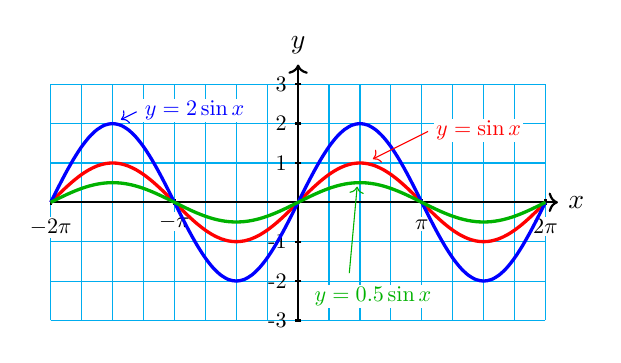
\begin{tikzpicture} [scale=1/2]
\draw[cyan] (-2*pi,-3) grid[xstep=pi/4, ystep=1] (2*pi,3);
\draw[black,thick,->](-2*pi,0)--(6.6,0) node[right]{$x$};
\draw[black,thick,->](0,-3)--(0,3.5) node[above]{$y$};
\foreach \y in {-3,-2,-1,1,2,3} \draw[black,thick] (0.08,\y)--++(-.16,0) node[left, scale=.8]{\y};
\draw[black,thick] (pi,.08)--++(0,-.16) node[below, yshift=-4, fill=white, inner sep=1, scale=.8] {$ \pi$};
\draw[black,thick] (2*pi,.08)--++(0,-.16) node[below, yshift=-4, fill=white, inner sep=1, scale=.8] {$ 2\pi$};
\draw[black,thick] (-pi,.08)--++(0,-.16) node[below, yshift=-2, fill=white, inner sep=1, scale=.8] {$ -\pi$};
\draw[black,thick] (-2*pi,.08)--++(0,-.16) node[below, yshift=-4, fill=white, inner sep=1, scale=.8] {$ -2\pi$};
\draw[samples=65, domain=-2*pi:2*pi, variable=\x, smooth,red, very thick] plot(\x,{sin(deg(\x))});
\draw[samples=65, domain=-2*pi:2*pi, variable=\x, smooth, blue, very thick] plot(\x,{2*sin(deg(\x))});
\draw[samples=65, domain=-2*pi:2*pi, variable=\x, smooth, green!70!black, very thick] plot(\x,{0.5*sin(deg(\x))});
\draw[red, <-] (1.9,1.1)--(3.3,1.8) node[above right, xshift=2, yshift=-4, fill=white, inner sep=1, scale=.8] {$y=\sin x$};
\draw[blue, <-] (-4.5,2.1)--(-4.1,2.3) node[above right, xshift=2, yshift=-4, fill=white, inner sep=1, scale=.8] {$y=2\sin x$};
\draw[green!70!black, <-] (1.5,0.4)--(1.3,-1.8) node[below, xshift=.3cm, yshift=-4, fill=white, inner sep=1, scale=.8] {$y=0.5\sin x$};
\end{tikzpicture}
\newline


exam7-1-2 transformations of cosine

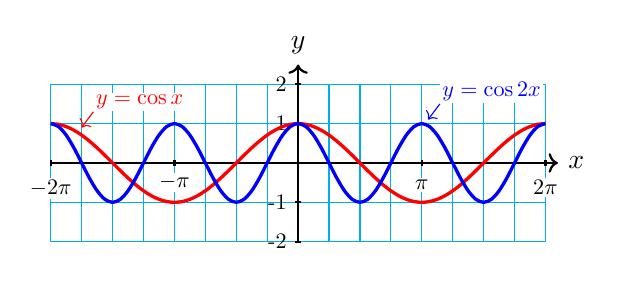
\begin{tikzpicture} [scale=1/2]
\draw[cyan] (-2*pi,-2) grid[xstep=pi/4, ystep=1] (2*pi,2);
\draw[black,thick,->](-2*pi,0)--(6.6,0) node[right]{$x$};
\draw[black,thick,->](0,-2)--(0,2.5) node[above]{$y$};
\foreach \y in {-2,-1,1,2} \draw[black,thick] (0.08,\y)--++(-.16,0) node[left, scale=.8]{\y};
\draw[black,thick] (pi,.08)--++(0,-.16) node[below, yshift=-4, fill=white, inner sep=1, scale=.8] {$ \pi$};
\draw[black,thick] (2*pi,.08)--++(0,-.16) node[below, yshift=-4, fill=white, inner sep=1, scale=.8] {$ 2\pi$};
\draw[black,thick] (-pi,.08)--++(0,-.16) node[below, yshift=-2, fill=white, inner sep=1, scale=.8] {$ -\pi$};
\draw[black,thick] (-2*pi,.08)--++(0,-.16) node[below, yshift=-4, fill=white, inner sep=1, scale=.8] {$ -2\pi$};
\draw[samples=65, domain=-2*pi:2*pi, variable=\x, smooth,red, very thick] plot(\x,{cos(deg(\x))});
\draw[samples=65, domain=-2*pi:2*pi, variable=\x, smooth, blue, very thick] plot(\x,{cos(deg(2*\x))});
\draw[red, <-] (-5.5,0.9)--++(0.3,0.4) node[above right, fill=white, inner sep=1, scale=.8] {$y=\cos x$};
\draw[blue, <-] (3.3,1.1)--++(0.3,0.4) node[above right, fill=white, inner sep=1, scale=.8] {$y=\cos 2x$};
\end{tikzpicture}
\newline


exam7-1-2also transformations of cosine

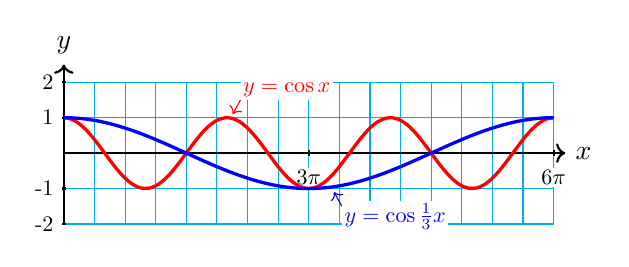
\begin{tikzpicture} [xscale=.33,yscale=.45]
\draw[cyan] (0,-2) grid[xstep=3*pi/8, ystep=1] (6*pi,2);
\draw[black,thick,->](0,0)--(19.3,0) node[right]{$x$};
\draw[black,thick,->](0,-2)--(0,2.5) node[above]{$y$};
\foreach \y in {-2,-1,1,2} \draw[black,thick] (0.08,\y)--++(-.16,0) node[left, scale=.8]{\y};
\draw[black,thick] (3*pi,.08)--++(0,-.16) node[below, yshift=-4, fill=white, inner sep=1, scale=.8] {$ 3\pi$};
\draw[black,thick] (6*pi,.08)--++(0,-.16) node[below, yshift=-4, fill=white, inner sep=1, scale=.8] {$ 6\pi$};
\draw[samples=65, domain=0:6*pi, variable=\x, smooth,red, very thick] plot(\x,{cos(deg(\x))});
\draw[samples=65, domain=0:6*pi, variable=\x, smooth, blue, very thick] plot(\x,{cos(deg(\x/3))});
\draw[red, <-] (6.5,1.1)--++(0.3,0.4) node[above right, fill=white, inner sep=1, scale=.8] {$y=\cos x$};
\draw[blue, <-] (10.4,-1.1)--++(0.3,-0.4) node[below right, yshift=2, fill=white, inner sep=1, scale=.8] {$y=\cos \frac{1}{3}x$};
\end{tikzpicture}
\newline


exam7-1-3 transformations of sine

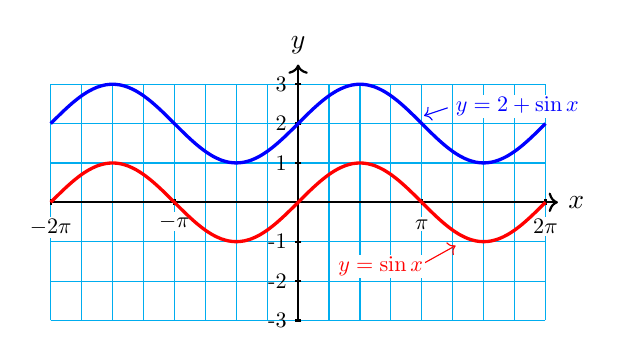
\begin{tikzpicture} [scale=1/2]
\draw[cyan] (-2*pi,-3) grid[xstep=pi/4, ystep=1] (2*pi,3);
\draw[black,thick,->](-2*pi,0)--(6.6,0) node[right]{$x$};
\draw[black,thick,->](0,-3)--(0,3.5) node[above]{$y$};
\foreach \y in {-3,-2,-1,1,2,3} \draw[black,thick] (0.08,\y)--++(-.16,0) node[left, scale=.8]{\y};
\draw[black,thick] (pi,.08)--++(0,-.16) node[below, yshift=-4, fill=white, inner sep=1, scale=.8] {$ \pi$};
\draw[black,thick] (2*pi,.08)--++(0,-.16) node[below, yshift=-4, fill=white, inner sep=1, scale=.8] {$ 2\pi$};
\draw[black,thick] (-pi,.08)--++(0,-.16) node[below, yshift=-2, fill=white, inner sep=1, scale=.8] {$ -\pi$};
\draw[black,thick] (-2*pi,.08)--++(0,-.16) node[below, yshift=-4, fill=white, inner sep=1, scale=.8] {$ -2\pi$};
\draw[samples=65, domain=-2*pi:2*pi, variable=\x, smooth,red, very thick] plot(\x,{sin(deg(\x))});
\draw[samples=65, domain=-2*pi:2*pi, variable=\x, smooth, blue, very thick] plot(\x,{2+sin(deg(\x))});
\draw[red, <-] (4,-1.1)--++(-0.9,-0.5) node[below left, xshift=2, yshift=4, fill=white, inner sep=1, scale=.8] {$y=\sin x$};
\draw[blue, <-] (3.2,2.2)--++(0.6,0.2) node[above right, xshift=2, yshift=-4, fill=white, inner sep=1, scale=.8] {$y=2+\sin x$};
\end{tikzpicture}
\newline


exam7-1-4 transformations of cosine

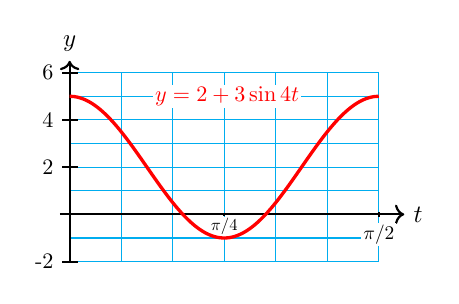
\begin{tikzpicture} [xscale=2.5, yscale=.3]
\draw[cyan] (0,-2) grid[xstep=pi/12, ystep=1] (pi/2,6);
\draw[black,thick,->](-0.05,0)--(1.7,0) node[right, scale=.9]{$t$};
\draw[black,thick,->](0,-2)--(0,6.5) node[above, scale=.9]{$y$};
\foreach \y in {-2, 2, 4, 6} \draw[black,thick] (0.04,\y)--++(-.08,0) node[left, scale=.8]{\y};
\draw[black,thick] (pi/4,.07)--++(0,-.14) node[below, fill=white, inner sep=1, scale=.6] {$ \pi/4$};
\draw[black,thick] (pi/2,.1)--++(0,-.2) node[below, yshift=-2, fill=white, inner sep=1, scale=.7] {$ \pi/2$};
\draw[samples=65, domain=0:pi/2, variable=\x, smooth, red, very thick] plot(\x,{2+3*cos(deg(4*\x))});
\node[text=red, fill=white, inner sep=1, scale=.8] at (.8,5) {$y=2+3\sin 4t$};
\end{tikzpicture}
\newline


exer7-1-4 grid

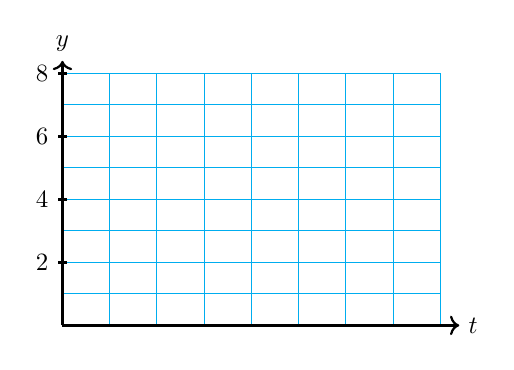
\begin{tikzpicture} [xscale=.6, yscale=.4]
\draw[cyan] (0,0) grid (8,8);
\draw[black,thick,->] (0,0)--(8.4,0) node[right, scale=0.9] {$t$};
\draw[black,thick,->] (0,0)--(0,8.4) node[above, scale=0.9] {$y$};
\foreach \y in {2,4,6,8} \draw[black,thick] (.1,\y)--++(-.2,0) node[left, scale=.9] {\y};
\end{tikzpicture}
\newline


exer7-1-4ans transformed sine

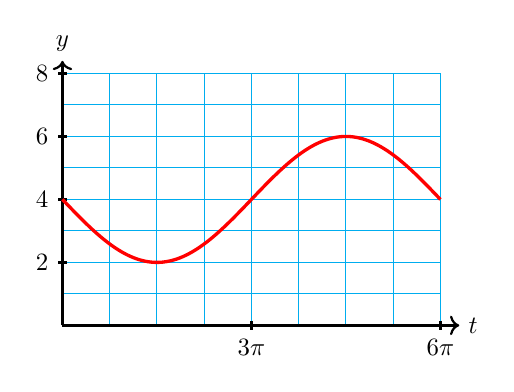
\begin{tikzpicture} [xscale=.6, yscale=.4]
\draw[cyan] (0,0) grid (8,8);
\draw[black,thick,->] (0,0)--(8.4,0) node[right, scale=0.9] {$t$};
\draw[black,thick,->] (0,0)--(0,8.4) node[above, scale=0.9] {$y$};
\foreach \y in {2,4,6,8} \draw[black,thick] (.1,\y)--++(-.2,0) node[left, scale=.9] {\y};
\draw[black, thick] (4,.15)--++(0,-.3) node[below, scale=.9]{$3\pi$};
\draw[black, thick] (8,.15)--++(0,-.3) node[below, scale=.9]{$6\pi$};
\draw[samples=65, domain=0:8, smooth, variable=\x, red, very thick] plot({\x},{4-2*sin(\x*45)});
\end{tikzpicture}
\newline


exam7-1-5 sinusoidal blood pressure

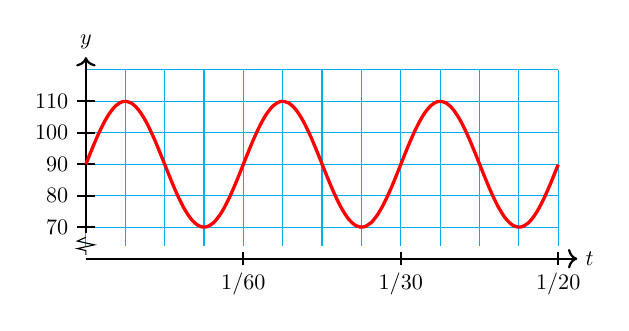
\begin{tikzpicture} [xscale=120, yscale=1/25]
\draw[cyan] (0,64) grid[xstep=1/240, ystep=10] (1/20,120);
\draw[black,thick,->] (0,60)--++(.052,0) node[right, scale=0.8] {$t$};
\draw[black,thick,->] (0,68)--(0,124) node[above, scale=0.8] {$y$};
\foreach \y in {70,80,90,...,110} \draw[black,thick] (.001,\y)--++(-.002,0) node[left, scale=.8] {\y};
\foreach \x in {1/60, 1/30, 1/20} \draw[black,thick] (\x,62)--++(0,-4) node[below, scale=.8] {\x};
\draw[black] (0,65)++(0,1.8)--++(-.0009, -1.2)--++(.0018,-1.2)--++(-.0018,-1.2)--++(.0009,-.6) -- ++(0, -1.4);

\draw[samples=64, domain=0:1/20, smooth, variable=\x, red, very thick] plot({\x},{90+20*sin(\x*60*360)});
\end{tikzpicture}
\newline


fig7-1a 3 sin 2x

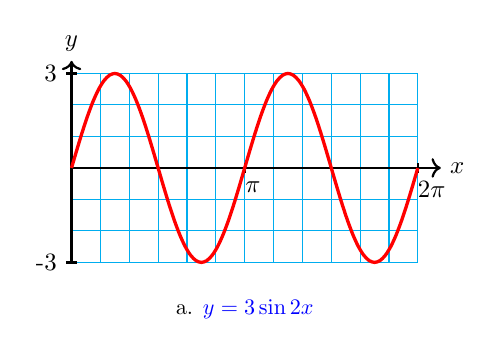
\begin{tikzpicture} [xscale=.7, yscale=.4]
\draw[cyan] (0,-3) grid[xstep=pi/6] (2*pi,3);
\draw[black,thick,->] (0,0)--(6.7,0) node[right, scale=0.9] {$x$};
\draw[black,thick,->] (0,-3)--(0,3.4) node[above, scale=0.9] {$y$};
\foreach \y in {-3,3} \draw[black,thick] (.1,\y)--++(-.2,0) node[left, scale=.9] {\y};
\draw[black, thick] (pi,.15)--++(0,-.3) node[below, xshift=3, scale=.9]{$\pi$};
\draw[black, thick] (2*pi,.15)--++(0,-.3) node[below, xshift=5, scale=.9]{$2\pi$};
\draw[samples=65, domain=0:2*pi, smooth, variable=\x, red, very thick] plot({\x},{3*sin(deg(\x*2))});
\node[scale=.8] at(pi,-4.5) {a.  $\color{blue}y=3\sin 2x$};
\end{tikzpicture}
\newline


fig7-1b -3 sin 2x

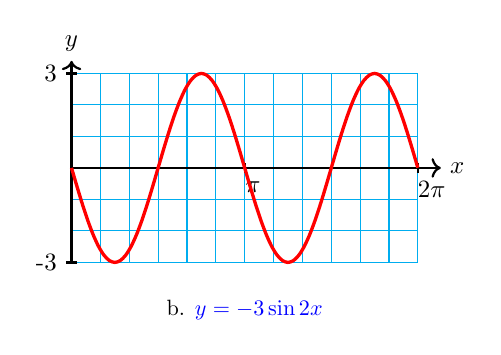
\begin{tikzpicture} [xscale=.7, yscale=.4]
\draw[cyan] (0,-3) grid[xstep=pi/6] (2*pi,3);
\draw[black,thick,->] (0,0)--(6.7,0) node[right, scale=0.9] {$x$};
\draw[black,thick,->] (0,-3)--(0,3.4) node[above, scale=0.9] {$y$};
\foreach \y in {-3,3} \draw[black,thick] (.1,\y)--++(-.2,0) node[left, scale=.9] {\y};
\draw[black, thick] (pi,.15)--++(0,-.3) node[below, xshift=3, scale=.9]{$\pi$};
\draw[black, thick] (2*pi,.15)--++(0,-.3) node[below, xshift=5, scale=.9]{$2\pi$};
\draw[samples=65, domain=0:2*pi, smooth, variable=\x, red, very thick] plot({\x},{-3*sin(deg(\x*2))});
\node[scale=.8] at(pi,-4.5) {b.  $\color{blue}y=-3\sin 2x$};
\end{tikzpicture}
\newline


fig7-1c 3 cos 2x

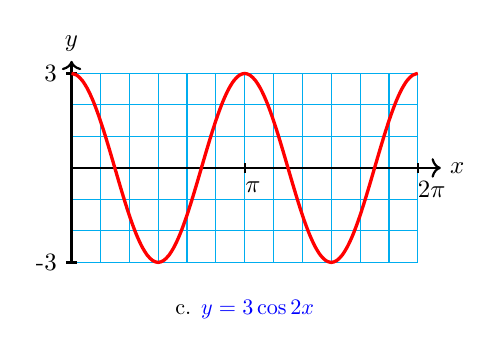
\begin{tikzpicture} [xscale=.7, yscale=.4]
\draw[cyan] (0,-3) grid[xstep=pi/6] (2*pi,3);
\draw[black,thick,->] (0,0)--(6.7,0) node[right, scale=0.9] {$x$};
\draw[black,thick,->] (0,-3)--(0,3.4) node[above, scale=0.9] {$y$};
\foreach \y in {-3,3} \draw[black,thick] (.1,\y)--++(-.2,0) node[left, scale=.9] {\y};
\draw[black, thick] (pi,.15)--++(0,-.3) node[below, xshift=3, scale=.9]{$\pi$};
\draw[black, thick] (2*pi,.15)--++(0,-.3) node[below, xshift=5, scale=.9]{$2\pi$};
\draw[samples=65, domain=0:2*pi, smooth, variable=\x, red, very thick] plot({\x},{3*cos(deg(\x*2))});
\node[scale=.8] at(pi,-4.5) {c.  $\color{blue}y=3\cos 2x$};
\end{tikzpicture}
\newline


fig7-1d -3 cos 2x

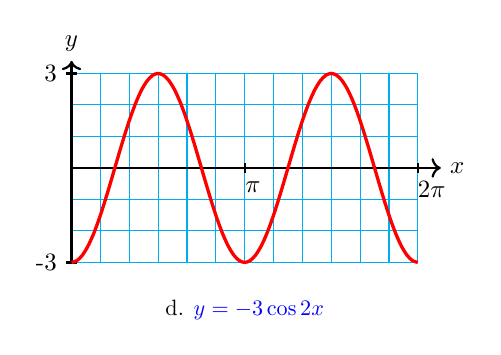
\begin{tikzpicture} [xscale=.7, yscale=.4]
\draw[cyan] (0,-3) grid[xstep=pi/6] (2*pi,3);
\draw[black,thick,->] (0,0)--(6.7,0) node[right, scale=0.9] {$x$};
\draw[black,thick,->] (0,-3)--(0,3.4) node[above, scale=0.9] {$y$};
\foreach \y in {-3,3} \draw[black,thick] (.1,\y)--++(-.2,0) node[left, scale=.9] {\y};
\draw[black, thick] (pi,.15)--++(0,-.3) node[below, xshift=3, scale=.9]{$\pi$};
\draw[black, thick] (2*pi,.15)--++(0,-.3) node[below, xshift=5, scale=.9]{$2\pi$};
\draw[samples=65, domain=0:2*pi, smooth, variable=\x, red, very thick] plot({\x},{-3*cos(deg(\x*2))});
\node[scale=.8] at(pi,-4.5) {d.  $\color{blue}y=-3\cos 2x$};
\end{tikzpicture}
\newline


exer7-1-5 sinusoidal voltage

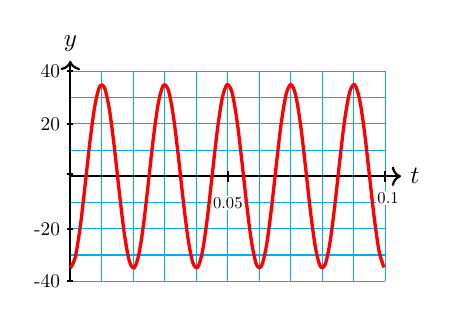
\begin{tikzpicture} [xscale=40, yscale=1/30]
\draw[cyan] (0,-40) grid[xstep=0.01, ystep=10] (0.1,40);
\draw[black,thick,->] (0,0)--(0.105,0) node[right, scale=0.9] {$t$};
\draw[black,thick,->] (0,-40)--(0,44) node[above, scale=0.9] {$y$};
\foreach \y in {-40,-20, 20,,40} \draw[black,thick] (.001,\y)--++(-.002,0) node[left, scale=.7] {\y};
\draw[black, thick] (0.05,2.1)--++(0,-4.2) node[below, yshift=-5, fill=white, inner sep=1, scale=.6]{$0.05$};
\draw[black, thick] (0.1,2.1)--++(0,-4.2) node[below, xshift=1, yshift=-3, fill=white, inner sep=1, scale=.6]{$0.1$};

\draw[samples=65, domain=0:0.1, smooth, variable=\x, red, very thick] plot({\x},{-35*cos(deg(100*pi*\x))});
\end{tikzpicture}
\newline


exam7-1-6 transformed tangent 

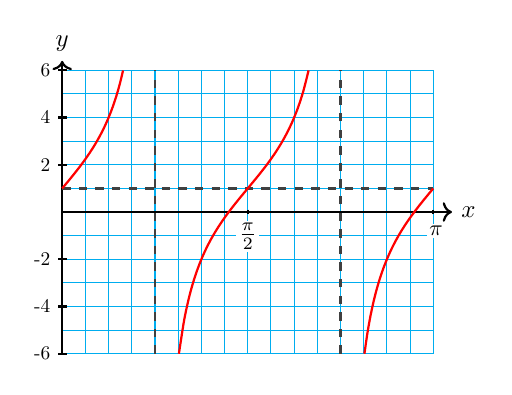
\begin{tikzpicture} [xscale=1.5, yscale=.3]
\draw[cyan] (0,-6) grid[xstep=pi/16] (pi,6);
\draw[black,thick,->] (0,0)--(3.3,0) node[right, scale=0.9] {$x$};
\draw[black,thick,->] (0,-6)--(0,6.4) node[above, scale=0.9] {$y$};
\foreach \y in {-6,-4,-2,2,4,6} \draw[black,thick] (.04,\y)--++(-.08,0) node[left, scale=.7] {\y};
\draw[black, thick] (pi/2,.1)--++(0,-.2) node[below, yshift=-2, fill=white, inner sep=1, scale=.9]{$ \frac{\pi}{2} $};
\draw[black, thick] (pi,.1)--++(0,-.2) node[below, xshift=1, yshift=-3, fill=white, inner sep=1, scale=.8]{$\pi$};
\draw[gray!50!black,thick,dashed] (pi/4,-6)--++(0,12);
\draw[gray!50!black,thick,dashed] (3*pi/4,-6)--++(0,12);
\draw[gray!50!black,thick,dashed] (0,1)--++(pi,0);
\draw[domain=0:{atan(5/3)/2*pi/180}, smooth, variable=\x, red, thick] plot({\x},{1+3*tan(deg(2*\x))});
\draw[domain={-atan(7/3)/2*pi/180}:{atan(5/3)/2*pi/180}, smooth, variable=\x, red, thick] plot({\x+pi/2},{1+3*tan(deg(2*\x))});
\draw[domain={-atan(7/3)/2*pi/180}:{0}, smooth, variable=\x, red, thick] plot({\x+pi},{1+3*tan(deg(2*\x))});
\end{tikzpicture}
\newline


exer7-1-6 transformed tangent -3+2tan pi x

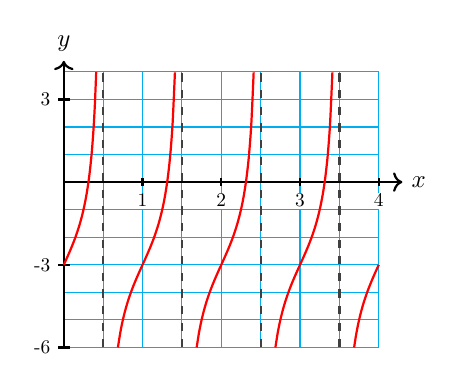
\begin{tikzpicture} [xscale=1, yscale=.35]
\draw[cyan] (0,-6) grid[xstep=1/2] (4,4);
\draw[black,thick,->] (0,0)--(4.3,0) node[right, scale=0.9] {$x$};
\draw[black,thick,->] (0,-6)--(0,4.4) node[above, scale=0.9] {$y$};
\foreach \y in {-6,-3,3} \draw[black,thick] (.08,\y)--++(-.16,0) node[left, scale=.7] {\y};
\foreach \x in {1,2,3,4} \draw[black,thick] (\x,.15)--++(0,-.3) node[below, yshift=-2, fill=white, inner sep=1, scale=.7] {\x};
\draw[gray!50!black,thick,dashed] (1/2,-6)--++(0,10);
\draw[gray!50!black,thick,dashed] (3/2,-6)--++(0,10);
\draw[gray!50!black,thick,dashed] (5/2,-6)--++(0,10);
\draw[gray!50!black,thick,dashed] (7/2,-6)--++(0,10);
\draw[domain=0:{atan(7/2)/180}, smooth, variable=\x, red, thick] plot({\x},{-3+2*tan(180*\x)});
\draw[domain={1-atan(3/2)/180}:{1+atan(7/2)/180}, smooth, variable=\x, red, thick] plot({\x},{-3+2*tan(180*\x)});
\draw[domain={2-atan(3/2)/180}:{2+atan(7/2)/180}, smooth, variable=\x, red, thick] plot({\x},{-3+2*tan(180*\x)});
\draw[domain={3-atan(3/2)/180}:{3+atan(7/2)/180}, smooth, variable=\x, red, thick] plot({\x},{-3+2*tan(180*\x)});
\draw[domain={4-atan(3/2)/180}:{4}, smooth, variable=\x, red, thick] plot({\x},{-3+2*tan(180*\x)});
\end{tikzpicture}
\newline


hp7-1-9ans transformed sine

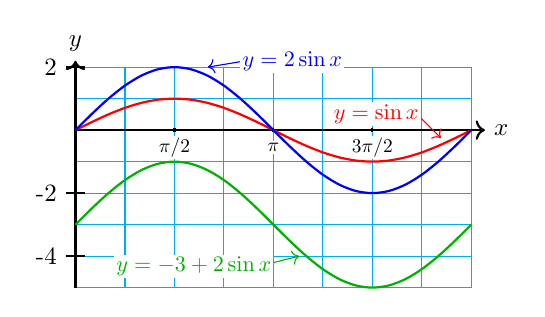
\begin{tikzpicture} [xscale=.8,yscale=.4]
\draw[cyan] (0,-5) grid[xstep=pi/4] (2*pi,2);
\draw[black,thick,->] (0,0)--(6.5,0) node[right, scale=.9]{$x$};
\draw[black,thick,->] (0,-5)--(0,2.2) node[above,scale=.9] {$y$};
\foreach \y in {-4,-2,2} \draw[black,thick] (.15,\y)--++(-.3,0) node[left,scale=.9]{\y};
\draw[black,thick] (pi/2,.07)--++(0,-.14) node[below, yshift=-1, fill=white, inner sep=1, scale=.7]{$\pi/2$};
\draw[black,thick] (pi,.07)--++(0,-.14) node[below, yshift=-3, fill=white, inner sep=1, scale=.7]{$\pi$};
\draw[black,thick] (3*pi/2,.07)--++(0,-.14) node[below, yshift=-1, fill=white, inner sep=1, scale=.7]{$3\pi/2$};
\draw[domain=0:2*pi, smooth, variable=\x,red, thick] plot({\x},{sin(deg(\x))});
\draw[domain=0:2*pi, smooth, variable=\x,blue, thick] plot({\x},{2*sin(deg(\x))});
\draw[domain=0:2*pi, smooth, variable=\x,green!70!black, thick] plot({\x},{-3+2*sin(deg(\x))});
\draw[red, <-] (5.8,-.25)--++(-0.4,0.8) node[below left, xshift=2, yshift=4, fill=white, inner sep=1, scale=.8] {$y=\sin x$};
\draw[blue, <-] (2.1,2)--++(0.6,0.2) node[right, xshift=-2, fill=white, inner sep=1, scale=.8] {$y=2\sin x$};
\draw[green!70!black, <-] (3.55,-4)--++(-0.4,-0.2) node[below left, yshift=3, fill=white, inner sep=1, scale=.8] {$y=-3+2\sin x$};
\end{tikzpicture}
\newline


hp7-1-11ans transformed cosine

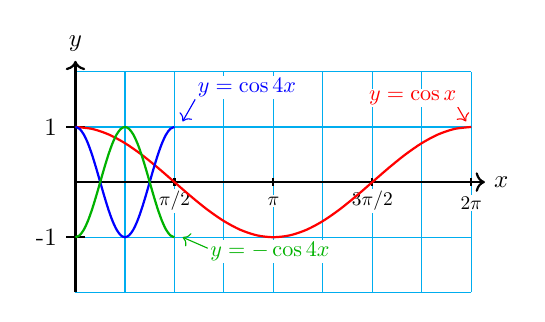
\begin{tikzpicture} [xscale=.8,yscale=.7]
\draw[cyan] (0,-2) grid[xstep=pi/4] (2*pi,2);
\draw[black,thick,->] (0,0)--(6.5,0) node[right, scale=.9]{$x$};
\draw[black,thick,->] (0,-2)--(0,2.2) node[above,scale=.9] {$y$};
\foreach \y in {-1,1} \draw[black,thick] (.15,\y)--++(-.3,0) node[left,scale=.9]{\y};
\draw[black,thick] (pi/2,.07)--++(0,-.14) node[below, yshift=-1, fill=white, inner sep=1, scale=.7]{$\pi/2$};
\draw[black,thick] (pi,.07)--++(0,-.14) node[below, yshift=-3, fill=white, inner sep=1, scale=.7]{$\pi$};
\draw[black,thick] (3*pi/2,.07)--++(0,-.14) node[below, yshift=-1, fill=white, inner sep=1, scale=.7]{$3\pi/2$};
\draw[domain=0:2*pi, smooth, variable=\x,red, thick] plot({\x},{cos(deg(\x))});
\draw[black,thick] (2*pi,.07)--++(0,-.14) node[below, yshift=-3, fill=white, inner sep=1, scale=.7]{$2\pi$};
\draw[domain=0:pi/2, smooth, variable=\x,blue, thick] plot({\x},{cos(deg(4*\x))});
\draw[domain=0:pi/2, smooth, variable=\x,green!70!black, thick] plot({\x},{-cos(deg(4*\x))});
\draw[red, <-] (6.2,1.1)--++(-0.2,0.4) node[below left, xshift=2, yshift=4, fill=white, inner sep=1, scale=.8] {$y=\cos x$};
\draw[blue, <-] (1.7,1.1)--++(0.2,0.4) node[above right, fill=white, inner sep=1, scale=.8] {$y=\cos 4x$};
\draw[green!70!black, <-] (1.7,-1)--++(0.4,-0.2) node[below right, yshift=3, fill=white, inner sep=1, scale=.8] {$y=-\cos 4x$};
\end{tikzpicture}
\newline


hp7-1-13ans transformed sine

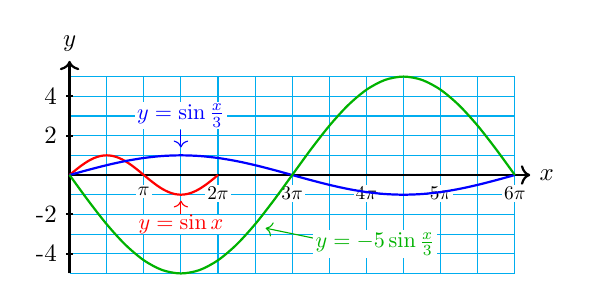
\begin{tikzpicture} [xscale=.3,yscale=.25]
\draw[cyan] (0,-5) grid[xstep=pi/2] (6*pi,5);
\draw[black,thick,->] (0,0)--(19.5,0) node[right, scale=.9]{$x$};
\draw[black,thick,->] (0,-5)--(0,5.8) node[above,scale=.9] {$y$};
\foreach \y in {-4,-2,2,4} \draw[black,thick] (.15,\y)--++(-.3,0) node[left,scale=.9]{\y};
\draw[black,thick] (pi,.07)--++(0,-.14) node[below, yshift=-3, fill=white, inner sep=1, scale=.7]{$\pi$};
\draw[black,thick] (2*pi,.07)--++(0,-.14) node[below, yshift=-3, fill=white, inner sep=1, scale=.7]{$2\pi$};
\draw[black,thick] (3*pi,.07)--++(0,-.14) node[below, yshift=-3, fill=white, inner sep=1, scale=.7]{$3\pi$};
\draw[black,thick] (4*pi,.07)--++(0,-.14) node[below, yshift=-3, fill=white, inner sep=1, scale=.7]{$4\pi$};
\draw[black,thick] (5*pi,.07)--++(0,-.14) node[below, yshift=-3, fill=white, inner sep=1, scale=.7]{$5\pi$};
\draw[black,thick] (6*pi,.07)--++(0,-.14) node[below, yshift=-3, fill=white, inner sep=1, scale=.7]{$6\pi$};
\draw[domain=0:2*pi, smooth, variable=\x,red, thick] plot({\x},{sin(deg(\x))});
\draw[domain=0:6*pi, smooth, variable=\x,blue, thick] plot({\x},{sin(deg(\x/3))});
\draw[domain=0:6*pi, smooth, variable=\x,green!70!black, thick] plot({\x},{-5*sin(deg(\x/3))});
\draw[red, <-] (3*pi/2,-1.3)--++(-0.,-0.7) node[below, yshift=-0, fill=white, inner sep=0, scale=.8] {$y=\sin x$};
\draw[blue, <-] (3*pi/2,1.4)--++(0.0,0.9) node[above , fill=white, inner sep=1, scale=.8] {$y=\sin \frac{x}{3}$};
\draw[green!70!black, <-] (8.3,-2.7)--++(2,-0.5) node[below right, yshift=3, fill=white, inner sep=1, scale=.8] {$y=-5\sin \frac{x}{3}$};
\end{tikzpicture}
\newline


hp7-1-15ans transformed cosine

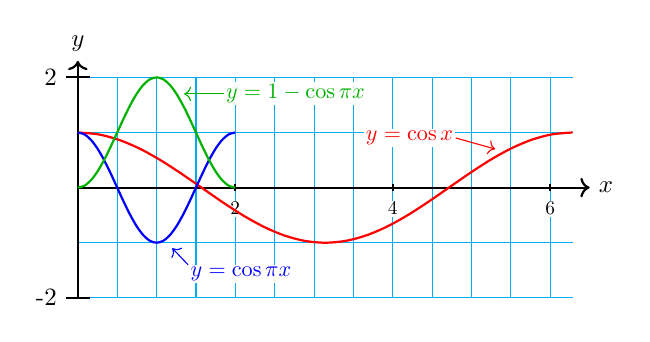
\begin{tikzpicture} [xscale=1,yscale=.7]
\draw[cyan] (0,-2) grid[xstep=1/2] (2*pi,2);
\draw[black,thick,->] (0,0)--(6.5,0) node[right, scale=.9]{$x$};
\draw[black,thick,->] (0,-2)--(0,2.3) node[above,scale=.9] {$y$};
\foreach \y in {-2,2} \draw[black,thick] (.15,\y)--++(-.3,0) node[left,scale=.9]{\y};
\foreach \x in {2,4,6} \draw[black,thick] (\x,.07)--++(0,-.14) node[below, yshift=-3, fill=white, inner sep=1, scale=.7]{\x};
\draw[domain=0:2*pi, smooth, variable=\x,red, thick] plot({\x},{cos(deg(\x))});
\draw[domain=0:2, smooth, variable=\x,blue, thick] plot({\x},{cos(deg(\x*pi))});
\draw[domain=0:2, smooth, variable=\x,green!70!black, thick] plot({\x},{1-cos(deg(\x*pi))});
\draw[red, <-] (5.3,.7)--++(-0.5,0.2) node[left, yshift=-0,fill=white, inner sep=1, scale=.8] {$y=\cos x$};
\draw[blue, <-] (1.2,-1.1)--++(0.2,-0.3) node[below right, fill=white, inner sep=1, scale=.8] {$y=\cos \pi x$};
\draw[green!70!black, <-] (1.35,1.7)--++(.5,-0.) node[ right,fill=white, inner sep=1, scale=.8] {$y=1- \cos \pi x$};
\end{tikzpicture}
\newline


hp7-1-17 transformed sine

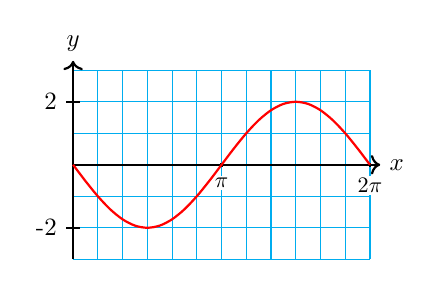
\begin{tikzpicture} [xscale=.6,yscale=.4]
\draw[cyan] (0,-3) grid[xstep=pi/6] (2*pi,3);
\draw[black,thick,->] (0,0)--(6.5,0) node[right, scale=.9]{$x$};
\draw[black,thick,->] (0,-3)--(0,3.3) node[above,scale=.9] {$y$};
\foreach \y in {-2,2} \draw[black,thick] (.15,\y)--++(-.3,0) node[left,scale=.9]{\y};
\draw[black,thick] (pi,.07)--++(0,-.14) node[below, yshift=-3, fill=white, inner sep=1, scale=.8]{$\pi$};
\draw[black,thick] (2*pi,.07)--++(0,-.14) node[below, yshift=-3, fill=white, inner sep=1, scale=.8]{$2\pi$};
\draw[domain=0:2*pi, smooth, variable=\x,red, thick] plot({\x},{-2*sin(deg(\x))});
\end{tikzpicture}
\newline


hp7-1-18 transformed cosine

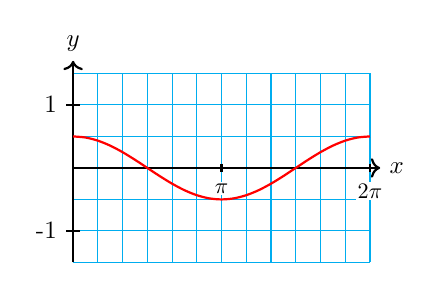
\begin{tikzpicture} [xscale=.6,yscale=.8]
\draw[cyan] (0,-3/2) grid[xstep=pi/6,ystep=1/2] (2*pi,3/2);
\draw[black,thick,->] (0,0)--(6.5,0) node[right, scale=.9]{$x$};
\draw[black,thick,->] (0,-3/2)--(0,1.7) node[above,scale=.9] {$y$};
\foreach \y in {-1,1} \draw[black,thick] (.15,\y)--++(-.3,0) node[left,scale=.9]{\y};
\draw[black,thick] (pi,.07)--++(0,-.14) node[below, yshift=-3, fill=white, inner sep=1, scale=.8]{$\pi$};
\draw[black,thick] (2*pi,.07)--++(0,-.14) node[below, yshift=-3, fill=white, inner sep=1, scale=.8]{$2\pi$};
\draw[domain=0:2*pi, smooth, variable=\x,red, thick] plot({\x},{1/2*cos(deg(\x))});
\end{tikzpicture}
\newline


hp7-1-19 transformed cosine

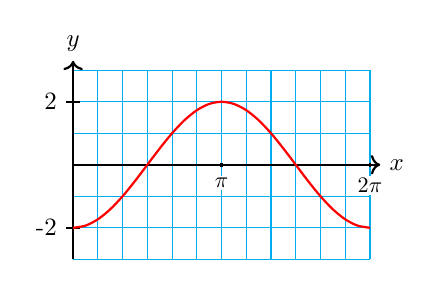
\begin{tikzpicture} [xscale=.6,yscale=.4]
\draw[cyan] (0,-3) grid[xstep=pi/6] (2*pi,3);
\draw[black,thick,->] (0,0)--(6.5,0) node[right, scale=.9]{$x$};
\draw[black,thick,->] (0,-3)--(0,3.3) node[above,scale=.9] {$y$};
\foreach \y in {-2,2} \draw[black,thick] (.15,\y)--++(-.3,0) node[left,scale=.9]{\y};
\draw[black,thick] (pi,.07)--++(0,-.14) node[below, yshift=-3, fill=white, inner sep=1, scale=.8]{$\pi$};
\draw[black,thick] (2*pi,.07)--++(0,-.14) node[below, yshift=-3, fill=white, inner sep=1, scale=.8]{$2\pi$};
\draw[domain=0:2*pi, smooth, variable=\x,red, thick] plot({\x},{-2*cos(deg(\x))});
\end{tikzpicture}
\newline


hp7-1-20 transformed sine

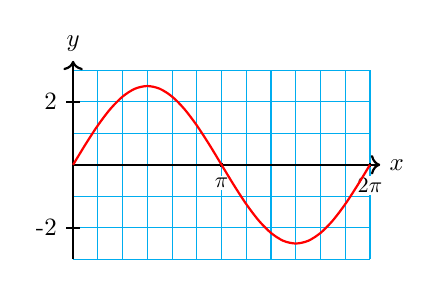
\begin{tikzpicture} [xscale=.6,yscale=.4]
\draw[cyan] (0,-3) grid[xstep=pi/6] (2*pi,3);
\draw[black,thick,->] (0,0)--(6.5,0) node[right, scale=.9]{$x$};
\draw[black,thick,->] (0,-3)--(0,3.3) node[above,scale=.9] {$y$};
\foreach \y in {-2,2} \draw[black,thick] (.15,\y)--++(-.3,0) node[left,scale=.9]{\y};
\draw[black,thick] (pi,.07)--++(0,-.14) node[below, yshift=-3, fill=white, inner sep=1, scale=.8]{$\pi$};
\draw[black,thick] (2*pi,.07)--++(0,-.14) node[below, yshift=-3, fill=white, inner sep=1, scale=.8]{$2\pi$};
\draw[domain=0:2*pi, smooth, variable=\x,red, thick] plot({\x},{2.5*sin(deg(\x))});
\end{tikzpicture}
\newline


hp7-1-21 transformed cosine

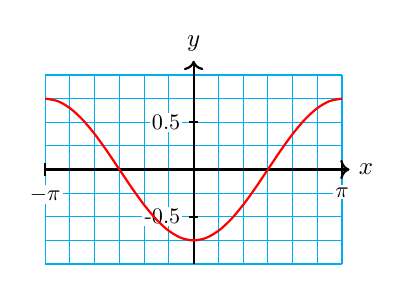
\begin{tikzpicture} [xscale=.6,yscale=1.2]
\draw[cyan] (-pi,-1) grid[xstep=pi/6, ystep=1/4] (pi,1);
\draw[black,thick,->] (-pi,0)--(3.3,0) node[right, scale=.9]{$x$};
\draw[black,thick,->] (0,-1)--(0,1.15) node[above,scale=.9] {$y$};
\foreach \y in {-0.5,0.5} \draw[black,thick] (.1,\y)--++(-.2,0) node[left, xshift=-2, fill=white, inner sep=1,scale=.8]{\y};
\draw[black,thick] (pi,.07)--++(0,-.14) node[below, yshift=-3, fill=white, inner sep=1, scale=.8]{$\pi$};
\draw[black,thick] (-pi,.07)--++(0,-.14) node[below, yshift=-3, fill=white, inner sep=1, scale=.8]{$-\pi$};
\draw[domain=-pi:pi, smooth, variable=\x,red, thick] plot({\x},{-0.75*cos(deg(\x))});
\end{tikzpicture}
\newline


hp7-1-22 transformed cosine

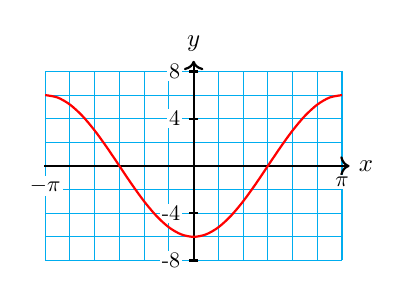
\begin{tikzpicture} [xscale=.6,yscale=.15]
\draw[cyan] (-pi,-8) grid[xstep=pi/6, ystep=2] (pi,8);
\draw[black,thick,->] (-pi,0)--(3.3,0) node[right, scale=.9]{$x$};
\draw[black,thick,->] (0,-8)--(0,8.9) node[above,scale=.9] {$y$};
\foreach \y in {-8,-4,4,8} \draw[black,thick] (.1,\y)--++(-.2,0) node[left, xshift=-2, fill=white, inner sep=1,scale=.8]{\y};
\draw[black,thick] (pi,.1)--++(0,-.1) node[below, yshift=-3, fill=white, inner sep=1, scale=.8]{$\pi$};
\draw[black,thick] (-pi,.1)--++(0,-.2) node[below, yshift=-3, fill=white, inner sep=1, scale=.8]{$-\pi$};
\draw[domain=-pi:pi, smooth, variable=\x,red, thick] plot({\x},{-6*cos(deg(\x))});
\end{tikzpicture}
\newline


hp7-1-23 transformed sine

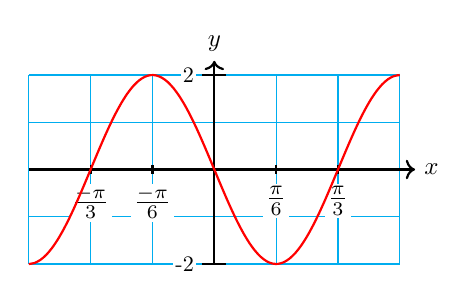
\begin{tikzpicture} [xscale=1.5,yscale=.6]
\draw[cyan] (-pi/2,-2) grid[xstep=pi/6, ystep=1] (pi/2,2);
\draw[black,thick,->] (-pi/2,0)--(1.7,0) node[right, scale=.9]{$x$};
\draw[black,thick,->] (0,-2)--(0,2.3) node[above,scale=.9] {$y$};
\foreach \y in {-2,2} \draw[black,thick] (.1,\y)--++(-.2,0) node[left, xshift=-2, fill=white, inner sep=1,scale=.8]{\y};
\draw[black,thick] (-pi/3,.1)--++(0,-.2) node[below, yshift=-3, fill=white, inner sep=1, scale=1]{$\frac{-\pi}{3}$};
\draw[black,thick] (-pi/6,.1)--++(0,-.2) node[below, yshift=-3, fill=white, inner sep=1, scale=1]{$\frac{-\pi}{6}$};
\draw[black,thick] (pi/3,.1)--++(0,-.2) node[below, yshift=-3, fill=white, inner sep=1, scale=1]{$\frac{\pi}{3}$};
\draw[black,thick] (pi/6,.1)--++(0,-.2) node[below, yshift=-3, fill=white, inner sep=1, scale=1]{$\frac{\pi}{6}$};
\draw[samples=65,domain=-pi/2:pi/2, smooth, variable=\x,red, thick] plot({\x},{-2*sin(deg(3*\x))});
\end{tikzpicture}
\newline


hp7-1-24 transformed sine

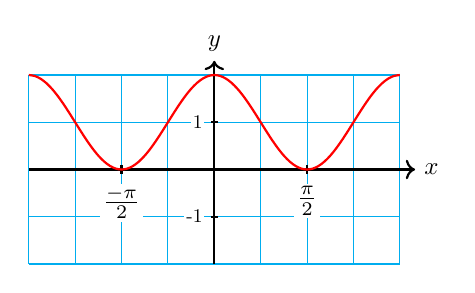
\begin{tikzpicture} [xscale=.75,yscale=.6]
\draw[cyan] (-pi,-2) grid[xstep=pi/4, ystep=1] (pi,2);
\draw[black,thick,->] (-pi,0)--(3.4,0) node[right, scale=.9]{$x$};
\draw[black,thick,->] (0,-2)--(0,2.3) node[above,scale=.9] {$y$};
\foreach \y in {-1,1} \draw[black,thick] (.06,\y)--++(-.12,0) node[left, xshift=-2, fill=white, inner sep=1,scale=.7]{\y};
\draw[black,thick] (-pi/2,.1)--++(0,-.2) node[below, yshift=-3, fill=white, inner sep=1, scale=1]{$\frac{-\pi}{2}$};
\draw[black,thick] (pi/2,.1)--++(0,-.2) node[below, yshift=-3, fill=white, inner sep=1, scale=1]{$\frac{\pi}{2}$};
\draw[samples=65,domain=-pi:pi, smooth, variable=\x,red, thick] plot({\x},{1+cos(deg(2*\x))});
\end{tikzpicture}
\newline


hp7-1-25 transformed sine

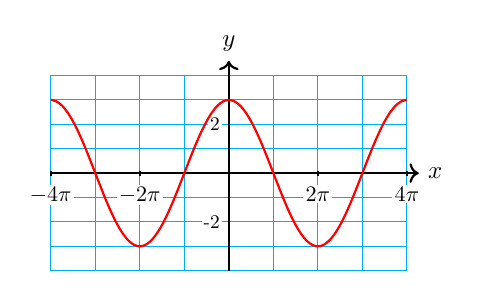
\begin{tikzpicture} [xscale=.18,yscale=.31]
\draw[cyan] (-4*pi,-4) grid[xstep=pi, ystep=1] (4*pi,4);
\draw[black,thick,->] (-4*pi,0)--(13.4,0) node[right, scale=.9]{$x$};
\draw[black,thick,->] (0,-4)--(0,4.6) node[above,scale=.9] {$y$};
\foreach \y in {-2,2} \draw[black,thick] (.06,\y)--++(-.12,0) node[left, xshift=-2, fill=white, inner sep=1,scale=.7]{\y};
\draw[black,thick] (-4*pi,.1)--++(0,-.2) node[below, yshift=-3, fill=white, inner sep=1, scale=.8]{$-4\pi$};
\draw[black,thick] (-2*pi,.1)--++(0,-.2) node[below, yshift=-3, fill=white, inner sep=1, scale=.8]{$-2\pi$};
\draw[black,thick] (2*pi,.1)--++(0,-.2) node[below, yshift=-3, fill=white, inner sep=1, scale=.8]{$2\pi$};
\draw[black,thick] (4*pi,.1)--++(0,-.2) node[below, yshift=-3, fill=white, inner sep=1, scale=.8]{$4\pi$};
\draw[samples=65,domain=-4*pi:4*pi, smooth, variable=\x,red, thick] plot({\x},{3*cos(deg(\x/2))});
\end{tikzpicture}
\newline


hp7-1-26 transformed cosine

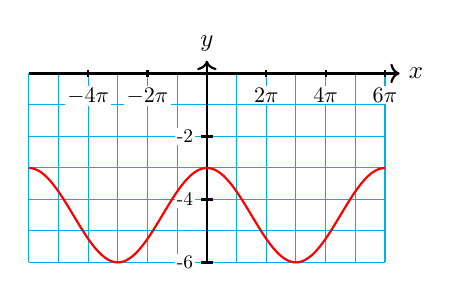
\begin{tikzpicture} [xscale=.12,yscale=.4]
\draw[cyan] (-6*pi,-6) grid[xstep=pi, ystep=1] (6*pi,0);
\draw[black,thick,->] (-6*pi,0)--(20.4,0) node[right, scale=.9]{$x$};
\draw[black,thick,->] (0,-6)--(0,.4) node[above,scale=.9] {$y$};
\foreach \y in {-2,-4,-6} \draw[black,thick] (.6,\y)--++(-1.2,0) node[left, xshift=-2, fill=white, inner sep=1,scale=.7]{\y};
\draw[black,thick] (-4*pi,.1)--++(0,-.2) node[below, yshift=-3, fill=white, inner sep=1, scale=.8]{$-4\pi$};
\draw[black,thick] (-2*pi,.1)--++(0,-.2) node[below, yshift=-3, fill=white, inner sep=1, scale=.8]{$-2\pi$};
\draw[black,thick] (2*pi,.1)--++(0,-.2) node[below, yshift=-3, fill=white, inner sep=1, scale=.8]{$2\pi$};
\draw[black,thick] (4*pi,.1)--++(0,-.2) node[below, yshift=-3, fill=white, inner sep=1, scale=.8]{$4\pi$};
\draw[black,thick] (6*pi,.1)--++(0,-.2) node[below, yshift=-3, fill=white, inner sep=1, scale=.8]{$6\pi$};
\draw[samples=65,domain=-6*pi:6*pi, smooth, variable=\x,red, thick] plot({\x},{-4.5+1.5*cos(deg(\x/3))});
\end{tikzpicture}
\newline


hp7-1-27 transformed cosine

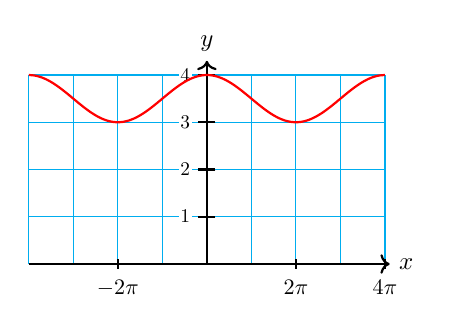
\begin{tikzpicture} [xscale=.18,yscale=.6]
\draw[cyan] (-4*pi,0) grid[xstep=pi, ystep=1] (4*pi,4);
\draw[black,thick,->] (-4*pi,0)--(12.9,0) node[right, scale=.9]{$x$};
\draw[black,thick,->] (0,0)--(0,4.3) node[above,scale=.9] {$y$};
\foreach \y in {1,2,3,4} \draw[black,thick] (.6,\y)--++(-1.2,0) node[left, xshift=-2, fill=white, inner sep=1,scale=.7]{\y};
\draw[black,thick] (-2*pi,.1)--++(0,-.2) node[below, yshift=-3, fill=white, inner sep=1, scale=.8]{$-2\pi$};
\draw[black,thick] (2*pi,.1)--++(0,-.2) node[below, yshift=-3, fill=white, inner sep=1, scale=.8]{$2\pi$};
\draw[black,thick] (4*pi,.1)--++(0,-.2) node[below, yshift=-3, fill=white, inner sep=1, scale=.8]{$4\pi$};
\draw[samples=65,domain=-4*pi:4*pi, smooth, variable=\x,red, thick] plot({\x},{3.5+.5*cos(deg(\x/2))});
\end{tikzpicture}
\newline


hp7-1-28 transformed sine

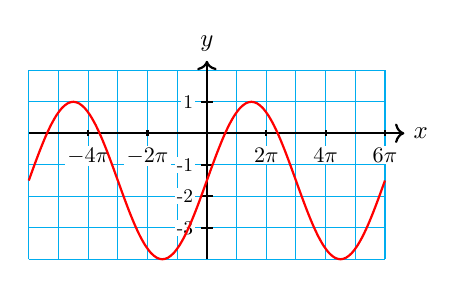
\begin{tikzpicture} [xscale=.12,yscale=.4]
\draw[cyan] (-6*pi,-4) grid[xstep=pi, ystep=1] (6*pi,2);
\draw[black,thick,->] (-6*pi,0)--(20.9,0) node[right, scale=.9]{$x$};
\draw[black,thick,->] (0,-4)--(0,2.3) node[above,scale=.9] {$y$};
\foreach \y in {-3,-2,-1,1} \draw[black,thick] (.6,\y)--++(-1.2,0) node[left, xshift=-2, fill=white, inner sep=1,scale=.7]{\y};
\draw[black,thick] (-4*pi,.1)--++(0,-.2) node[below, yshift=-3, fill=white, inner sep=1, scale=.8]{$-4\pi$};
\draw[black,thick] (-2*pi,.1)--++(0,-.2) node[below, yshift=-3, fill=white, inner sep=1, scale=.8]{$-2\pi$};
\draw[black,thick] (2*pi,.1)--++(0,-.2) node[below, yshift=-3, fill=white, inner sep=1, scale=.8]{$2\pi$};
\draw[black,thick] (4*pi,.1)--++(0,-.2) node[below, yshift=-3, fill=white, inner sep=1, scale=.8]{$4\pi$};
\draw[black,thick] (6*pi,.1)--++(0,-.2) node[below, yshift=-3, fill=white, inner sep=1, scale=.8]{$6\pi$};
\draw[samples=65,domain=-6*pi:6*pi, smooth, variable=\x,red, thick] plot({\x},{-1.5+2.5*sin(deg(\x/3))});
\end{tikzpicture}
\newline


hp7-1-29 transformed sine

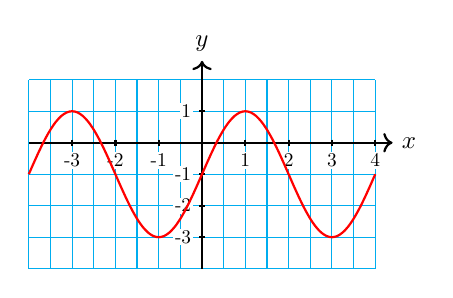
\begin{tikzpicture} [xscale=.55,yscale=.4]
\draw[cyan] (-4,-4) grid[xstep=1/2, ystep=1] (4,2);
\draw[black,thick,->] (-4,0)--(4.4,0) node[right, scale=.9]{$x$};
\draw[black,thick,->] (0,-4)--(0,2.6) node[above,scale=.9] {$y$};
\foreach \x in {-3,-2,-1,1,2,3,4} \draw[black,thick] (\x,.1)--++(0,-.2) node[below, yshift=-2, fill=white, inner sep=1,scale=.7]{\x};
\foreach \y in {-3,-2,-1,1} \draw[black,thick] (.06,\y)--++(-.12,0) node[left, xshift=-2, fill=white, inner sep=1,scale=.7]{\y};
\draw[samples=65,domain=-4:4, smooth, variable=\x,red, thick] plot({\x},{-1+2*sin(90*\x)});
\end{tikzpicture}
\newline


hp7-1-30 transformed cosine

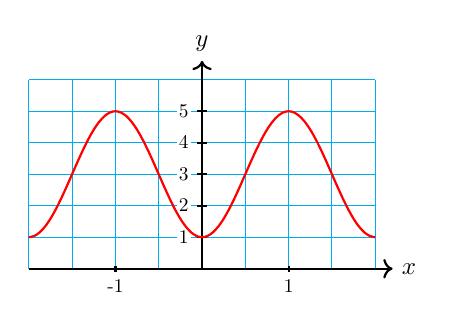
\begin{tikzpicture} [xscale=1.1,yscale=.4]
\draw[cyan] (-2,0) grid[xstep=1/2, ystep=1] (2,6);
\draw[black,thick,->] (-2,0)--(2.2,0) node[right, scale=.9]{$x$};
\draw[black,thick,->] (0,0)--(0,6.6) node[above,scale=.9] {$y$};
\foreach \x in {-1,1} \draw[black,thick] (\x,.1)--++(0,-.2) node[below, yshift=-2, fill=white, inner sep=1,scale=.7]{\x};
\foreach \y in {1,2,3,4,5} \draw[black,thick] (.06,\y)--++(-.12,0) node[left, xshift=-2, fill=white, inner sep=1,scale=.7]{\y};
\draw[samples=65,domain=-2:2, smooth, variable=\x,red, thick] plot({\x},{3-2*cos(180*\x)});
\end{tikzpicture}
\newline


hp7-1-grid
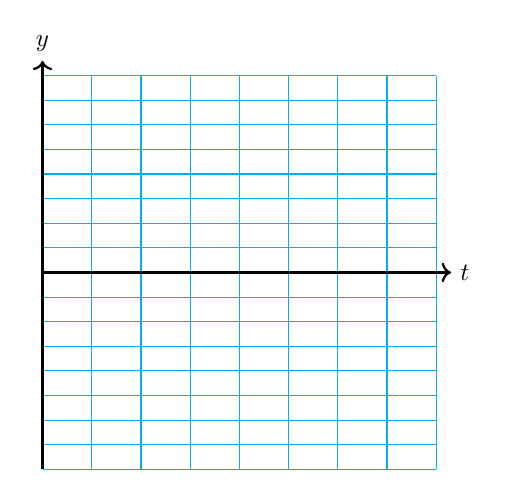
\begin{tikzpicture} [scale=5/8]
\draw[cyan] (0,-4) grid[ystep=1/2, xstep=1] (8,4);
\draw[black,thick,->] (0,0)--(8.3,0) node[right, scale=.9]{$t$};
\draw[black,thick,->] (0,-4)--(0,4.3) node[above, scale=.9]{$y$};
\end{tikzpicture}
\newline


hp7-1-31ans
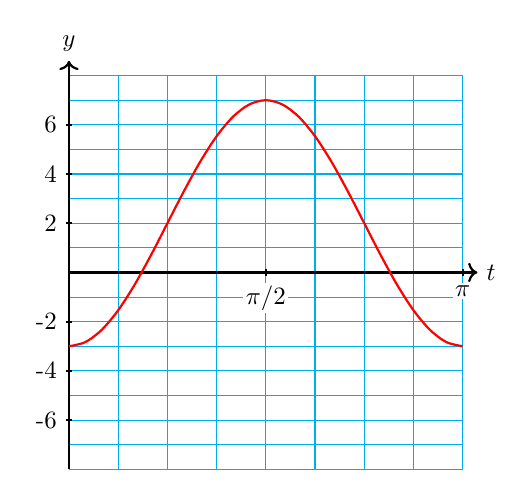
\begin{tikzpicture} [scale=5/8]
\draw[cyan] (0,-4) grid[ystep=1/2, xstep=1] (8,4);
\draw[black,thick,->] (0,0)--(8.3,0) node[right, scale=.9]{$t$};
\draw[black,thick,->] (0,-4)--(0,4.3) node[above, scale=.9]{$y$};
\foreach \y [evaluate=\y as \yi using int( \y /2 )] in {-6,-4,-2,2,4,6} \draw[black,thick] (.06,\yi)--++(-.12,0) node[left,scale=.9]{\y};
\draw[black,thick] (4,.08)--++(0,-.16) node[below, yshift=-2, fill=white, inner sep=1, scale=.9]{$\pi/2$};
\draw[black,thick] (8,.08)--++(0,-.16) node[below, yshift=-2, fill=white, inner sep=1, scale=.9]{$\pi$};
\draw[domain=0:8, smooth, variable=\x,red, thick] plot({\x},{1-2.5*cos(45*\x)});
\end{tikzpicture}
\newline


hp7-1-31ans
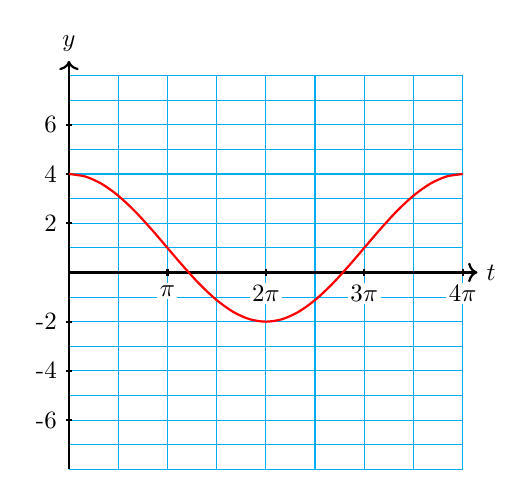
\begin{tikzpicture} [scale=5/8]
\draw[cyan] (0,-4) grid[ystep=1/2, xstep=1] (8,4);
\draw[black,thick,->] (0,0)--(8.3,0) node[right, scale=.9]{$t$};
\draw[black,thick,->] (0,-4)--(0,4.3) node[above, scale=.9]{$y$};
\foreach \y [evaluate=\y as \yi using int( \y /2 )] in {-6,-4,-2,2,4,6} \draw[black,thick] (.06,\yi)--++(-.12,0) node[left,scale=.9]{\y};
\draw[black,thick] (2,.08)--++(0,-.16) node[below, yshift=-2, fill=white, inner sep=1, scale=.9]{$\pi$};
\draw[black,thick] (4,.08)--++(0,-.16) node[below, yshift=-2, fill=white, inner sep=1, scale=.9]{$2\pi$};
\draw[black,thick] (6,.08)--++(0,-.16) node[below, yshift=-2, fill=white, inner sep=1, scale=.9]{$3\pi$};
\draw[black,thick] (8,.08)--++(0,-.16) node[below, yshift=-2, fill=white, inner sep=1, scale=.9]{$4\pi$};
\draw[domain=0:8, smooth, variable=\x,red, thick] plot({\x},{.5+1.5*cos(45*\x)});
\end{tikzpicture}
\newline


hp7-1-33ans
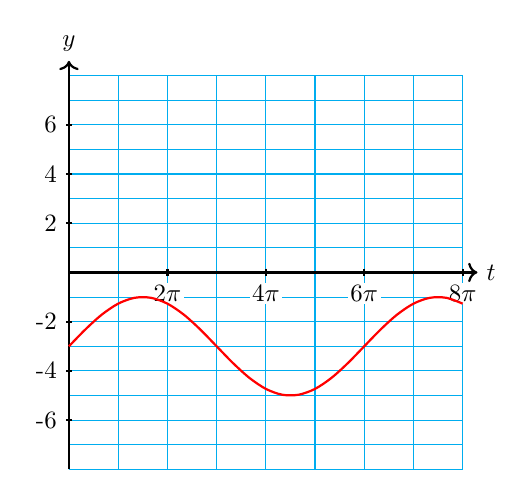
\begin{tikzpicture} [scale=5/8]
\draw[cyan] (0,-4) grid[ystep=1/2, xstep=1] (8,4);
\draw[black,thick,->] (0,0)--(8.3,0) node[right, scale=.9]{$t$};
\draw[black,thick,->] (0,-4)--(0,4.3) node[above, scale=.9]{$y$};
\foreach \y [evaluate=\y as \yi using int( \y /2 )] in {-6,-4,-2,2,4,6} \draw[black,thick] (.06,\yi)--++(-.12,0) node[left,scale=.9]{\y};
\draw[black,thick] (2,.08)--++(0,-.16) node[below, yshift=-2, fill=white, inner sep=1, scale=.9]{$2\pi$};
\draw[black,thick] (4,.08)--++(0,-.16) node[below, yshift=-2, fill=white, inner sep=1, scale=.9]{$4\pi$};
\draw[black,thick] (6,.08)--++(0,-.16) node[below, yshift=-2, fill=white, inner sep=1, scale=.9]{$6\pi$};
\draw[black,thick] (8,.08)--++(0,-.16) node[below, yshift=-2, fill=white, inner sep=1, scale=.9]{$8\pi$};
\draw[domain=0:8, smooth, variable=\x,red, thick] plot({\x},{-1.5+sin(60*\x)});
\end{tikzpicture}
\newline


hp7-1-37 transformed sine

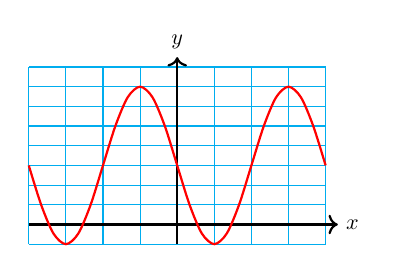
\begin{tikzpicture} [xscale=.6,yscale=.25]
\draw[cyan] (-pi,-1) grid[xstep=pi/4] (pi,8);
\draw[black,thick,->] (-pi,0)--(3.4,0) node[right,scale=.8]{$x$};
\draw[black,thick,->] (0,-1)--(0,8.5) node[above,scale=.8]{$y$};
\draw[domain=-pi:pi, smooth, variable=\x, red, thick] plot (\x,{3-4*sin(deg(2*\x))});
\end{tikzpicture}
\newline


hp7-1-37ans transformed sine

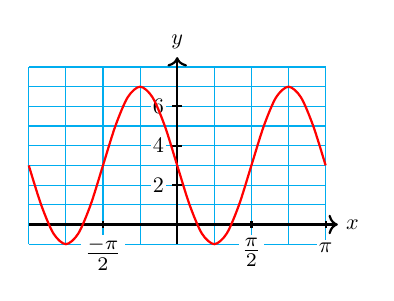
\begin{tikzpicture} [xscale=.6,yscale=.25]
\draw[cyan] (-pi,-1) grid[xstep=pi/4] (pi,8);
\draw[black,thick,->] (-pi,0)--(3.4,0) node[right,scale=.8]{$x$};
\draw[black,thick,->] (0,-1)--(0,8.5) node[above,scale=.8]{$y$};
\foreach \y in {2,4,6} \draw[black,thick] (.1,\y)--++(-.2,0) node[left, xshift=-2, fill=white, inner sep=1, scale=.8]{\y};
\draw[black,thick] (-pi/2,.2)--++(0,-.4) node[below,yshift=-2, fill=white, inner sep=1] {$\frac{-\pi}{2}$};
\draw[black,thick] (pi/2,.2)--++(0,-.4) node[below,yshift=-2, fill=white, inner sep=1] {$\frac{\pi}{2}$};
\draw[black,thick] (pi,.2)--++(0,-.4) node[below,yshift=-4, fill=white, inner sep=1, scale=.8] {$\pi$};
\draw[domain=-pi:pi, smooth, variable=\x, red, thick] plot (\x,{3-4*sin(deg(2*\x))});
\end{tikzpicture}
\newline


hp7-1-38 transformed cosine

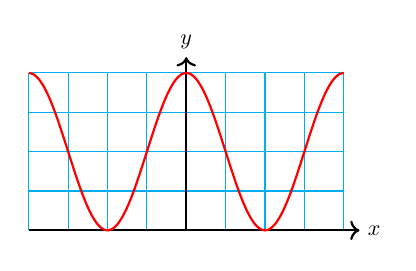
\begin{tikzpicture} [scale=.5]
\draw[cyan] (-4,0) grid (4,4);
\draw[black,thick,->] (-4,0)--(4.4,0) node[right,scale=.8]{$x$};
\draw[black,thick,->] (0,0)--(0,4.4) node[above,scale=.8]{$y$};
\draw[samples=65,domain=-4:4, smooth, variable=\x, red, thick] plot (\x,{2+2*cos(90*\x)});
\end{tikzpicture}
\newline


hp7-1-39 transformed sine

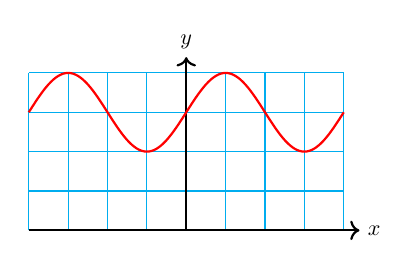
\begin{tikzpicture} [scale=.5]
\draw[cyan] (-4,0) grid (4,4);
\draw[black,thick,->] (-4,0)--(4.4,0) node[right,scale=.8]{$x$};
\draw[black,thick,->] (0,0)--(0,4.4) node[above,scale=.8]{$y$};
\draw[samples=65,domain=-4:4, smooth, variable=\x, red, thick] plot (\x,{3+1*sin(90*\x)});
\end{tikzpicture}
\newline


hp7-1-39ans transformed sine

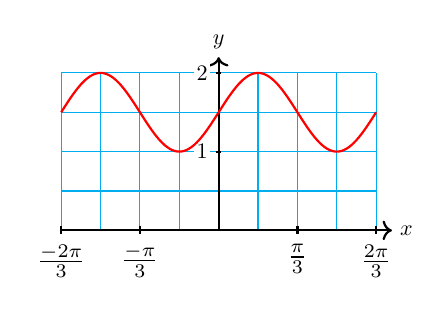
\begin{tikzpicture} [scale=.5]
\draw[cyan] (-4,0) grid (4,4);
\draw[black,thick,->] (-4,0)--(4.4,0) node[right,scale=.8]{$x$};
\draw[black,thick,->] (0,0)--(0,4.4) node[above,scale=.8]{$y$};
\foreach \y [evaluate=\y as \yi using int( \y *2 )] in {1,2} \draw[black,thick] (.06,\yi)--++(-.12,0) node[left, xshift=-2, fill=white, inner sep=1,scale=.8]{\y};
\draw[black,thick] (-4,.1)--++(0,-.2) node[below] {$\frac{-2\pi}{3}$};
\draw[black,thick] (-2,.1)--++(0,-.2) node[below] {$\frac{-\pi}{3}$};
\draw[black,thick] (2,.1)--++(0,-.2) node[below] {$\frac{\pi}{3}$};
\draw[black,thick] (4,.1)--++(0,-.2) node[below] {$\frac{2\pi}{3}$};
\draw[samples=65,domain=-4:4, smooth, variable=\x, red, thick] plot (\x,{3+1*sin(90*\x)});
\end{tikzpicture}
\newline


hp7-1-40 transformed cosine

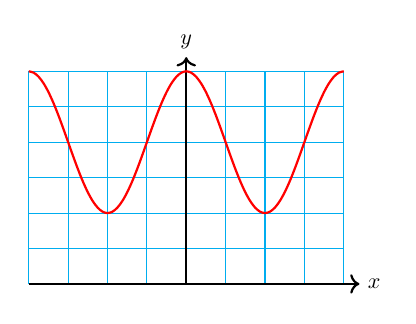
\begin{tikzpicture} [xscale=.5, yscale=.45]
\draw[cyan] (-4,0) grid (4,6);
\draw[black,thick,->] (-4,0)--(4.4,0) node[right,scale=.8]{$x$};
\draw[black,thick,->] (0,0)--(0,6.4) node[above,scale=.8]{$y$};
\draw[samples=65,domain=-4:4, smooth, variable=\x, red, thick] plot (\x,{4+2*cos(90*\x)});
\end{tikzpicture}
\newline


hp7-1-41 transformed sine

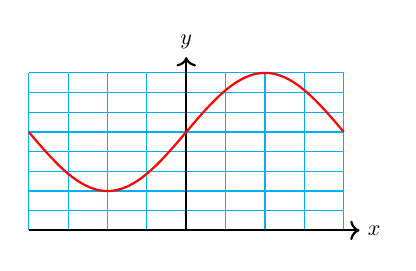
\begin{tikzpicture} [xscale=.5, yscale=.25]
\draw[cyan] (-4,0) grid (4,8);
\draw[black,thick,->] (-4,0)--(4.4,0) node[right,scale=.8]{$x$};
\draw[black,thick,->] (0,0)--(0,8.8) node[above,scale=.8]{$y$};
\draw[samples=65,domain=-4:4, smooth, variable=\x, red, thick] plot (\x,{5+3*sin(45*\x)});
\end{tikzpicture}
\newline


hp7-1-41ans transformed sine

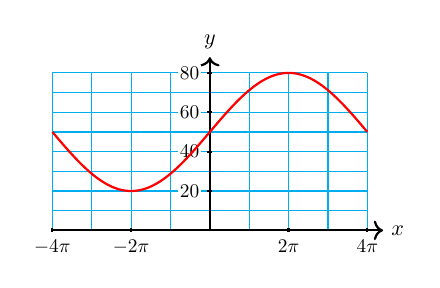
\begin{tikzpicture} [xscale=.5, yscale=.25]
\draw[cyan] (-4,0) grid (4,8);
\draw[black,thick,->] (-4,0)--(4.4,0) node[right,scale=.8]{$x$};
\draw[black,thick,->] (0,0)--(0,8.8) node[above,scale=.8]{$y$};
\foreach \y [evaluate=\y as \yi using int( \y *10 )] in {2,4,6,8} \draw[black,thick] (.06,\y)--++(-.12,0) node[left, xshift=-2, fill=white, inner sep=1,scale=.7]{\yi};
\draw[black,thick] (-4,.1)--++(0,-.2) node[below, scale=.7] {$-4\pi$};
\draw[black,thick] (-2,.1)--++(0,-.2) node[below, scale=.7] {$-2\pi$};
\draw[black,thick] (2,.1)--++(0,-.2) node[below, scale=.7] {$2\pi$};
\draw[black,thick] (4,.1)--++(0,-.2) node[below, scale=.7] {$4\pi$};
\draw[samples=65,domain=-4:4, smooth, variable=\x, red, thick] plot (\x,{5+3*sin(45*\x)});
\end{tikzpicture}
\newline


hp7-1-42 transformed cosine

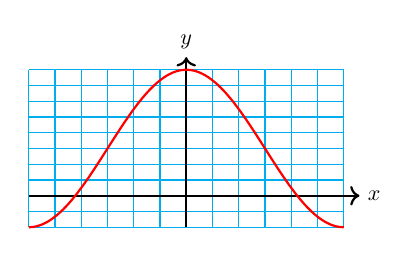
\begin{tikzpicture} [xscale=1/3, yscale=.2]
\draw[cyan] (-6,-2) grid (6,8);
\draw[black,thick,->] (-6,0)--(6.6,0) node[right,scale=.8]{$x$};
\draw[black,thick,->] (0,-2)--(0,8.8) node[above,scale=.8]{$y$};
\draw[samples=65,domain=-6:6, smooth, variable=\x, red, thick] plot (\x,{3+5*cos(30*\x)});
\end{tikzpicture}
\newline


hp7-1-43 transformed sine

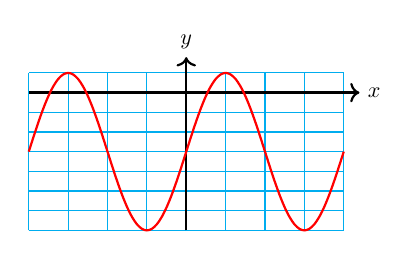
\begin{tikzpicture} [xscale=.5, yscale=.25]
\draw[cyan] (-4,-7) grid (4,1);
\draw[black,thick,->] (-4,0)--(4.4,0) node[right,scale=.8]{$x$};
\draw[black,thick,->] (0,-7)--(0,1.8) node[above,scale=.8]{$y$};
\draw[samples=65,domain=-4:4, smooth, variable=\x, red, thick] plot (\x,{-3+4*sin(90*\x)});
\end{tikzpicture}
\newline


hp7-1-43ans transformed sine

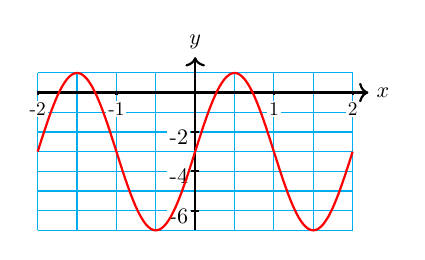
\begin{tikzpicture} [xscale=.5, yscale=.25]
\draw[cyan] (-4,-7) grid (4,1);
\draw[black,thick,->] (-4,0)--(4.4,0) node[right,scale=.8]{$x$};
\draw[black,thick,->] (0,-7)--(0,1.8) node[above,scale=.8]{$y$};
\foreach \x [evaluate=\x as \xi using int( \x /2 )] in {-4,-2,2,4} \draw[black,thick] (\x,.1)--++(0,-.2) node[below, yshift=-2, fill=white, inner sep=1,scale=.7]{\xi};
\foreach \y in {-6,-4,-2} \draw[black,thick] (.1,\y)--++(-.2,0) node[left, yshift=-2, fill=white, inner sep=1, scale=.8] {\y};
\draw[samples=65,domain=-4:4, smooth, variable=\x, red, thick] plot (\x,{-3+4*sin(90*\x)});
\end{tikzpicture}
\newline


hp7-1-44 transformed sine

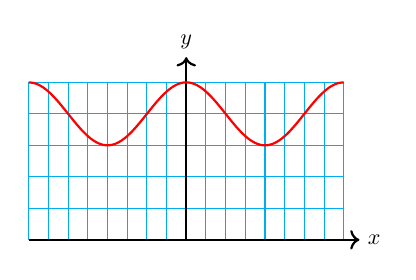
\begin{tikzpicture} [xscale=.5, yscale=.4]
\draw[cyan] (-4,0) grid[xstep=1/2] (4,5);
\draw[black,thick,->] (-4,0)--(4.4,0) node[right,scale=.8]{$x$};
\draw[black,thick,->] (0,0)--(0,5.8) node[above,scale=.8]{$y$};
\draw[samples=65,domain=-4:4, smooth, variable=\x, red, thick] plot (\x,{4+1*cos(90*\x)});
\end{tikzpicture}
\newline



hp7-1-45ans tide

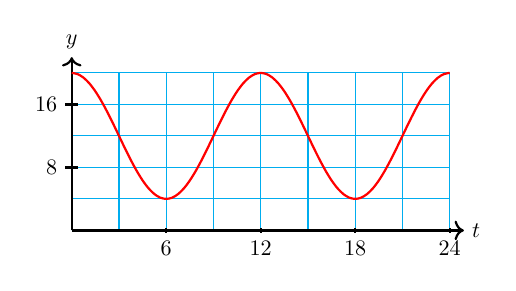
\begin{tikzpicture} [xscale=.2, yscale=.1]
\draw[cyan] (0,0) grid[xstep=3, ystep=4] (24,20);
\draw[black,thick,->] (0,0)--(24.9,0) node[right,scale=.8]{$t$};
\draw[black,thick,->] (0,0)--(0,22) node[above,scale=.8]{$y$};
\foreach \x in {6,12, 18,24} \draw[black,thick] (\x,.3)--++(0,-.6) node[below, scale=.8]{\x};
\foreach \y in {8,16} \draw[black,thick] (.4,\y)--++(-.8,0) node[left, scale=.8]{\y};
\draw[samples=65,domain=0:24, smooth, variable=\x, red, thick] plot (\x,{12+8*cos(30*\x)});
\end{tikzpicture}
\newline



hp7-1-47ans paddlewheel

\begin{tikzpicture} [xscale=.2, yscale=.1]
\draw[cyan] (0,-4) grid[xstep=5, ystep=4] (25,24);
\draw[black,thick,->] (0,0)--(25.9,0) node[right,scale=.8]{$t$};
\draw[black,thick,->] (0,-4)--(0,26) node[above,scale=.8]{$y$};
\foreach \x in {10,20} \draw[black,thick] (\x,.3)--++(0,-.6) node[below, scale=.8]{\x};
\foreach \y in {8,16,24} \draw[black,thick] (.4,\y)--++(-.8,0) node[left, scale=.8]{\y};
\draw[samples=65,domain=0:25, smooth, variable=\x, red, thick] plot (\x,{10+14*cos(36*\x)});
\end{tikzpicture}
\newline



hp7-1-49 daylight in Salt Lake

\begin{tikzpicture} [xscale=.2, yscale=.16]
\draw[cyan] (0,0) grid[xstep=6, ystep=5] (24,15);
\draw[black,thick,->] (0,0)--(24.9,0) node[right,scale=.8]{$t$};
\draw[black,thick,->] (0,0)--(0,15.9) node[above,scale=.8]{$y$};
\foreach \x in {6,12,18,24} \draw[black,thick] (\x,.3)--++(0,-.6) node[below, scale=.8]{\x};
\foreach \y in {5,10,15} \draw[black,thick] (.4,\y)--++(-.8,0) node[left, scale=.8]{\y};
\draw[samples=65,domain=0:24, smooth, variable=\x, red, thick] plot (\x,{12-2.4*cos(20*\x)});
\end{tikzpicture}
\newline



hp7-1-50 oscillating spring 

\begin{tikzpicture} [xscale=1.1, yscale=.25]
\draw[cyan] (0,0) grid[xstep=1, ystep=2] (4,10);
\draw[black,thick,->] (0,0)--(4.2,0) node[right,scale=.8]{$t$};
\draw[black,thick,->] (0,0)--(0,10.9) node[above,scale=.8]{$y$};
\foreach \x in {1,2,3,4} \draw[black,thick] (\x,.3)--++(0,-.6) node[below, scale=.8]{\x};
\foreach \y in {2,4,6,8,10} \draw[black,thick] (.04,\y)--++(-.08,0) node[left, scale=.8]{\y};
\draw[samples=65,domain=0:4, smooth, variable=\x, red, thick] plot (\x,{6.5-1.5*cos(180*\x)});
\end{tikzpicture}
\newline



hp7-1-51 voltage

\begin{tikzpicture} [xscale=1.2, yscale=.8]
\draw[cyan] (0,-2) grid[xstep=1, ystep=1] (5,2);
\draw[black,thick,->] (0,0)--(5.2,0) node[right,scale=.8]{$t$};
\draw[black,thick,->] (0,-2)--(0,2.2) node[above,scale=.8]{$y$};
\draw[black,thick] (5,.1)--++(0,-.2) node[below, yshift=-2, fill=white, inner sep=1, scale=.8] {0.05};
\foreach \y [evaluate=\y as \yi using int(100*\y)]  in {-2,-1,1,2} \draw[black,thick] (.04,\y)--++(-.08,0) node[left, scale=.8]{\yi};
\draw[samples=65,domain=0:5, smooth, variable=\x, red, thick] plot (\x,{1.55*cos(216*\x)});
\end{tikzpicture}
\newline



hp7-1-52 moon phases

\begin{tikzpicture} [xscale=.15, yscale=.25]
\draw[cyan] (0,0) grid[xstep=7, ystep=1] (28,10);
\draw[black,thick,->] (0,0)--(29.5,0) node[right,scale=.8]{$t$};
\draw[black,thick,->] (0,0)--(0,10.2) node[above,scale=.8]{$y$};
\foreach \y [evaluate=\y as \yi using int(10*\y)]  in {5,10} 
\draw[black,thick] (.04,\y)--++(-.08,0) node[left, scale=.8]{\yi};
\foreach \x in {7,14,21,28} \draw[black,thick] (\x,.3)--++(0,-.6) node[below, scale=.8]{\x};
\draw[samples=65,domain=0:28, smooth, variable=\x, red, thick] plot (\x,{5+5*cos(180*\x/7)});
\end{tikzpicture}
\newline



hp7-1-53ans tan 2x
\begin{tikzpicture} [xscale=1.5, yscale=.4]
\draw[cyan] (-pi/4,-3) grid[xstep=pi/8] (3*pi/4,3);
\draw[black,thick,->] (-pi/4,0)--(2.5,0) node[right,scale=.8]{$x$};
\draw[black,thick,->] (0,-3)--(0,3.4) node[above,scale=.8]{$y$};
\foreach \y [evaluate=\y as \yi using int(1*\y)]  in {-2,2} 
\draw[black,thick] (.04,\y)--++(-.08,0) node[left, xshift=-2, fill=white, inner sep=1, scale=.8]{\yi};
\draw[black,thick] (-pi/4,.1)--++(0,-.2) node[below, yshift=-2, fill=white, inner sep=1]{$\frac{-\pi}{4}$};
\draw[black,thick] (pi/4,.1)--++(0,-.2) node[below, yshift=-2, fill=white, inner sep=1]{$\frac{\pi}{4}$};
\draw[black,thick] (pi/2,.1)--++(0,-.2) node[below, yshift=-2, fill=white, inner sep=1]{$\frac{\pi}{2}$};
\draw[black,thick] (3*pi/4,.1)--++(0,-.2) node[below, yshift=-2, fill=white, inner sep=1]{$\frac{3\pi}{4}$};
\draw[samples=65,domain={atan(-3)/2}:{atan(3)/2}, smooth, variable=\x, red, thick] plot ({\x*pi/180},{tan(2*\x)});
\draw[samples=65,domain={atan(-3)/2}:{atan(3)/2}, smooth, variable=\x, red, thick] plot ({\x*pi/180+pi/2},{tan(2*\x)});
\end{tikzpicture}
\newline



hp7-1-55ans 4+2 tan 3x
\begin{tikzpicture} [xscale=2.2, yscale=.2]
\draw[cyan] (-pi/6,-4) grid[xstep=pi/12, ystep=2] (pi/2,12);
\draw[black,thick,->] (-pi/6,0)--(1.7,0) node[right,scale=.8]{$x$};
\draw[black,thick,->] (0,-3)--(0,12.9) node[above,scale=.8]{$y$};
\foreach \y in {-4,4,8,12} 
 \draw[black,thick] (.04,\y)--++(-.08,0) node[left, xshift=-2, fill=white, inner sep=1, scale=.8]{\y};
\draw[black,thick] (-pi/6,.1)--++(0,-.2) node[below, yshift=-2, fill=white, inner sep=1]{$\frac{-\pi}{6}$};
\draw[black,thick] (pi/6,.1)--++(0,-.2) node[below, yshift=-2, fill=white, inner sep=1]{$\frac{\pi}{6}$};
\draw[black,thick] (pi/3,.1)--++(0,-.2) node[below, yshift=-2, fill=white, inner sep=1]{$\frac{\pi}{3}$};
\draw[black,thick] (pi/2,.1)--++(0,-.2) node[below, yshift=-2, fill=white, inner sep=1]{$\frac{\pi}{2}$};
\draw[samples=65,domain={atan(-4)/3}:{atan(4)/3}, smooth, variable=\x, red, thick] plot ({\x*pi/180},{4+2*tan(3*\x)});
\draw[samples=65,domain={atan(-4)/3}:{atan(4)/3}, smooth, variable=\x, red, thick] plot ({\x*pi/180+pi/3},{4+2*tan(3*\x)});
\end{tikzpicture}
\newline



hp7-1-57ans 3- tan x/4
\begin{tikzpicture} [xscale=.2, yscale=.4]
\draw[cyan] (-2*pi,-1) grid[xstep=pi, ystep=1] (6*pi,7);
\draw[black,thick,->] (-2*pi,0)--(19.8,0) node[right,scale=.8]{$x$};
\draw[black,thick,->] (0,-1)--(0,7.6) node[above,scale=.8]{$y$};
\foreach \y in {2,4,6} 
 \draw[black,thick] (.2,\y)--++(-.4,0) node[left, xshift=-2, fill=white, inner sep=1, scale=.8]{\y};
\draw[black,thick] (-2*pi,.1)--++(0,-.2) node[below, yshift=-2, fill=white, inner sep=1, scale=.8]{$-2\pi$};
\draw[black,thick] (2*pi,.1)--++(0,-.2) node[below, yshift=-2, fill=white, inner sep=1, scale=.8]{$2\pi$};
\draw[black,thick] (4*pi,.1)--++(0,-.2) node[below, yshift=-2, fill=white, inner sep=1, scale=.8]{$4\pi$};
\draw[black,thick] (6*pi,.1)--++(0,-.2) node[below, yshift=-2, fill=white, inner sep=1, scale=.8]{$6\pi$};
\draw[samples=65,domain={atan(-4)*4}:{atan(4)*4}, smooth, variable=\x, red, thick] plot ({\x*pi/180},{3-tan(\x /4)});
\draw[samples=65,domain={atan(-4)*4}:{atan(4)*4}, smooth, variable=\x, red, thick] plot ({\x*pi/180+4*pi},{3-tan(\x /4)});
\end{tikzpicture}
\newline


hp7-1-59 3cos 4x
\begin{tikzpicture} [xscale=.8, yscale=.45]
\draw[cyan] (0,-3) grid[xstep=pi/12] (2*pi,3);
\draw[black,thick,->] (0,0)--(6.6,0) node[right, scale=.9] {$x$};
\draw[black,thick,->] (0,-3)--(0,3.4) node[above, scale=.9] {$y$};
\foreach \y in {-3,-2,-1,1,2,3} \draw[black,thick] (.08,\y)--++(-.16,0) node[left, scale=.8] {\y};
\draw[black,thick] (pi/2,.1)--++(0,-.2) node[below, yshift=-2, fill=white, inner sep=1]{$\frac{\pi}{2}$};
\draw[black,thick] (pi,.1)--++(0,-.2) node[below, yshift=-4, fill=white, inner sep=1, scale=.8]{$\pi$};
\draw[black,thick] (3*pi/2,.1)--++(0,-.2) node[below, yshift=-2, fill=white, inner sep=1]{$\frac{3\pi}{2}$};
\draw[black,thick] (2*pi,.1)--++(0,-.2) node[below, yshift=-4, fill=white, inner sep=1, scale=.8]{$2\pi$};
\draw[samples=65,domain=0:2*pi, smooth, variable=\x, red, thick] plot ({\x},{3*cos(deg(4*\x))});
\draw[blue,thick] (0,1.5) --++(2*pi,0);
\end{tikzpicture}
\newline


hp7-1-60 2sin 3x
\begin{tikzpicture} [xscale=.8, yscale=.45]
\draw[cyan] (0,-3) grid[xstep=pi/12] (2*pi,3);
\draw[black,thick,->] (0,0)--(6.6,0) node[right, scale=.9] {$x$};
\draw[black,thick,->] (0,-3)--(0,3.4) node[above, scale=.9] {$y$};
\foreach \y in {-3,-2,-1,1,2,3} \draw[black,thick] (.08,\y)--++(-.16,0) node[left, scale=.8] {\y};
\draw[black,thick] (pi/2,.1)--++(0,-.2) node[below, yshift=-2, fill=white, inner sep=1]{$\frac{\pi}{2}$};
\draw[black,thick] (pi,.1)--++(0,-.2) node[below, yshift=-4, fill=white, inner sep=1, scale=.8]{$\pi$};
\draw[black,thick] (3*pi/2,.1)--++(0,-.2) node[below, yshift=-2, fill=white, inner sep=1]{$\frac{3\pi}{2}$};
\draw[black,thick] (2*pi,.1)--++(0,-.2) node[below, yshift=-4, fill=white, inner sep=1, scale=.8]{$2\pi$};
\draw[samples=65,domain=0:2*pi, smooth, variable=\x, red, thick] plot ({\x},{2*sin(deg(3*\x))});
\draw[blue,very thick] ($ -sqrt(2)*(0,1) $) --++(2*pi,0);
\end{tikzpicture}
\newline


hp7-1-61 2+3 sin 2x
\begin{tikzpicture} [xscale=.8, yscale=.45]
\draw[cyan] (0,-1) grid[xstep=pi/12] (2*pi,5);
\draw[black,thick,->] (0,0)--(6.6,0) node[right, scale=.9] {$x$};
\draw[black,thick,->] (0,-1)--(0,5.4) node[above, scale=.9] {$y$};
\foreach \y in {2,4} \draw[black,thick] (.08,\y)--++(-.16,0) node[left, scale=.8] {\y};
\draw[black,thick] (pi/2,.1)--++(0,-.2) node[below, yshift=-2, fill=white, inner sep=1]{$\frac{\pi}{2}$};
\draw[black,thick] (pi,.1)--++(0,-.2) node[below, yshift=-4, fill=white, inner sep=1, scale=.8]{$\pi$};
\draw[black,thick] (3*pi/2,.1)--++(0,-.2) node[below, yshift=-2, fill=white, inner sep=1]{$\frac{3\pi}{2}$};
\draw[black,thick] (2*pi,.1)--++(0,-.2) node[below, yshift=-4, fill=white, inner sep=1, scale=.8]{$2\pi$};
\draw[samples=65,domain=0:2*pi, smooth, variable=\x, red, thick] plot ({\x},{2+3*sin(deg(2*\x))});
\draw[blue,very thick] (0,0.5) --++(2*pi,0);
\end{tikzpicture}
\newline


hp7-1-62 2+4 cos 2x
\begin{tikzpicture} [xscale=.8, yscale=.33]
\draw[cyan] (0,-2) grid[xstep=pi/12] (2*pi,6);
\draw[black,thick,->] (0,0)--(6.6,0) node[right, scale=.9] {$x$};
\draw[black,thick,->] (0,-2)--(0,6.6) node[above, scale=.9] {$y$};
\foreach \y in {-2,2,4,6} \draw[black,thick] (.09,\y)--++(-.18,0) node[left, scale=.8] {\y};
\draw[black,thick] (pi/2,.1)--++(0,-.2) node[below, yshift=-2, fill=white, inner sep=1]{$\frac{\pi}{2}$};
\draw[black,thick] (pi,.1)--++(0,-.2) node[below, yshift=-4, fill=white, inner sep=1, scale=.8]{$\pi$};
\draw[black,thick] (3*pi/2,.1)--++(0,-.2) node[below, yshift=-2, fill=white, inner sep=1]{$\frac{3\pi}{2}$};
\draw[black,thick] (2*pi,.1)--++(0,-.2) node[below, yshift=-4, fill=white, inner sep=1, scale=.8]{$2\pi$};
\draw[samples=65,domain=0:2*pi, smooth, variable=\x, red, thick] plot ({\x},{2+4*cos(deg(2*\x))});
\draw[blue,very thick] (0,4) --++(2*pi,0);
\end{tikzpicture}
\newline


hp7-1-63 -3+ tan 3x
\begin{tikzpicture} [xscale=.8, yscale=.25]
\draw[cyan] (0,-6) grid[xstep=pi/12] (2*pi,4);
\draw[black,thick,->] (0,0)--(6.6,0) node[right, scale=.9] {$x$};
\draw[black,thick,->] (0,-6)--(0,4.6) node[above, scale=.9] {$y$};
\foreach \y in {-6,-4,-2,2,4} \draw[black,thick] (.09,\y)--++(-.18,0) node[left, scale=.8] {\y};
\draw[black,thick] (pi/2,.1)--++(0,-.2) node[below, yshift=-2, fill=white, inner sep=1]{$\frac{\pi}{2}$};
\draw[black,thick] (pi,.1)--++(0,-.2) node[below, yshift=-4, fill=white, inner sep=1, scale=.8]{$\pi$};
\draw[black,thick] (3*pi/2,.1)--++(0,-.2) node[below, yshift=-2, fill=white, inner sep=1]{$\frac{3\pi}{2}$};
\draw[black,thick] (2*pi,.1)--++(0,-.2) node[below, yshift=-4, fill=white, inner sep=1, scale=.8]{$2\pi$};
\draw[samples=65,domain=0:{atan(7)/3*pi/180}, smooth, variable=\x, red, thick] plot ({\x},{-3+tan(deg(3*\x))});
\draw[samples=65,domain={atan(-3)/3*pi/180}:{atan(7)/3*pi/180}, smooth, variable=\x, red, thick] plot ({\x+pi/3},{-3+tan(deg(3*\x))});
\draw[samples=65,domain={atan(-3)/3*pi/180}:{atan(7)/3*pi/180}, smooth, variable=\x, red, thick] plot ({\x+2*pi/3},{-3+tan(deg(3*\x))});
\draw[samples=65,domain={atan(-3)/3*pi/180}:{atan(7)/3*pi/180}, smooth, variable=\x, red, thick] plot ({\x+pi},{-3+tan(deg(3*\x))});
\draw[samples=65,domain={atan(-3)/3*pi/180}:{atan(7)/3*pi/180}, smooth, variable=\x, red, thick] plot ({\x+4*pi/3},{-3+tan(deg(3*\x))});
\draw[samples=65,domain={atan(-3)/3*pi/180}:{atan(7)/3*pi/180}, smooth, variable=\x, red, thick] plot ({\x+5*pi/3},{-3+tan(deg(3*\x))});
\draw[samples=65,domain={atan(-3)/3*pi/180}:{0}, smooth, variable=\x, red, thick] plot ({\x+2*pi},{-3+tan(deg(3*\x))});
\draw[blue,very thick] (0,-2) --++(2*pi,0);
\end{tikzpicture}
\newline


hp7-1-64 2+ tan 4x
\begin{tikzpicture} [xscale=.8, yscale=.25]
\draw[cyan] (0,-2) grid[xstep=pi/12] (2*pi,8);
\draw[black,thick,->] (0,0)--(6.6,0) node[right, scale=.9] {$x$};
\draw[black,thick,->] (0,-2)--(0,8.6) node[above, scale=.9] {$y$};
\foreach \y in {-2,2,4,6,8} \draw[black,thick] (.09,\y)--++(-.18,0) node[left, scale=.8] {\y};
\draw[black,thick] (pi/2,.1)--++(0,-.2) node[below, yshift=-2, fill=white, inner sep=1]{$\frac{\pi}{2}$};
\draw[black,thick] (pi,.1)--++(0,-.2) node[below, yshift=-4, fill=white, inner sep=1, scale=.8]{$\pi$};
\draw[black,thick] (3*pi/2,.1)--++(0,-.2) node[below, yshift=-2, fill=white, inner sep=1]{$\frac{3\pi}{2}$};
\draw[black,thick] (2*pi,.1)--++(0,-.2) node[below, yshift=-4, fill=white, inner sep=1, scale=.8]{$2\pi$};
\draw[samples=65,domain=0:{atan(6)/4*pi/180}, smooth, variable=\x, red, thick] plot ({\x},{2+tan(deg(4*\x))});
\draw[samples=65,domain={atan(-4)/4*pi/180}:{atan(6)/4*pi/180}, smooth, variable=\x, red, thick] plot ({\x+pi/4},{2+tan(deg(4*\x))});
\draw[samples=65,domain={atan(-4)/4*pi/180}:{atan(6)/4*pi/180}, smooth, variable=\x, red, thick] plot ({\x+pi/2},{2+tan(deg(4*\x))});
\draw[samples=65,domain={atan(-4)/4*pi/180}:{atan(6)/4*pi/180}, smooth, variable=\x, red, thick] plot ({\x+3*pi/4},{2+tan(deg(4*\x))});
\draw[samples=65,domain={atan(-4)/4*pi/180}:{atan(6)/4*pi/180}, smooth, variable=\x, red, thick] plot ({\x+pi},{2+tan(deg(4*\x))});
\draw[samples=65,domain={atan(-4)/4*pi/180}:{atan(6)/4*pi/180}, smooth, variable=\x, red, thick] plot ({\x+5*pi/4},{2+tan(deg(4*\x))});
\draw[samples=65,domain={atan(-4)/4*pi/180}:{atan(6)/4*pi/180}, smooth, variable=\x, red, thick] plot ({\x+3*pi/2},{2+tan(deg(4*\x))});
\draw[samples=65,domain={atan(-4)/4*pi/180}:{atan(6)/4*pi/180}, smooth, variable=\x, red, thick] plot ({\x+7*pi/4},{2+tan(deg(4*\x))});
\draw[samples=65,domain={atan(-4)/4*pi/180}:{0}, smooth, variable=\x, red, thick] plot ({\x+2*pi},{2+tan(deg(4*\x))});
\draw[blue,very thick] (0,3) --++(2*pi,0);
\end{tikzpicture}
\newline




\end{document}
